\chapter{年羹尧和皇十四子}
% 原书第269页

康熙五十七年（1718）二月，突然传来了西藏拉藏汗的求救信，说准噶尔军队已经开始围攻拉萨。\NoteRef{07}{1}这时的康熙正在病中挣扎，同时还在为第三次立储之事烦心。前一年夏天，他曾收到过军报，称准噶尔派军队从新疆方向进入西藏，但他根据已有情报，认为拉萨自己的兵力完全有能力防守，因而并未发兵去往西藏。这封突如其来的求救信，显示出事态严峻，使得康熙和朝廷的注意力从持续了半年的立储之事转到了西部用兵上面。


% 原书第269–270页

从带兵打仗的角度来说，康熙前半生有两大引以为傲的战绩。一是平定南方，这包括平定三藩和收复台湾；二是三次西征，战胜了准噶尔部的噶尔丹。但由于西北地域辽阔，民族构成复杂，又远离清朝的政治经济中心，清朝对西北的实际控制比较薄弱。噶尔丹兵败去世以后，策妄阿喇布坦成为了准噶尔各部的最强者。策妄阿喇布坦在中文、俄文和藏文史料中都曾出现，是一代枭雄，但关于他的生平，各方却都没有专门的记录，现在所知都是从各方史料中拼凑出来的。\NoteRef{07}{2}雍正登基后，曾派遣使臣去见策妄阿喇布坦，使臣回来后写有长篇的出使汇报，其中概述了策妄阿喇布坦年轻时的经历：他很小的时候父亲被杀，作为孤儿被噶尔丹收养，但后来噶尔丹杀了他的弟弟，霸占了要嫁给他的女子，他便带着人逃跑了。\NoteRef{07}{3}1690年代，在噶尔丹与康熙大战之际，策妄阿喇布坦数次偷袭了噶尔丹的老巢科布多。在康熙西征与噶尔丹决战时，策妄阿喇布坦便顺势吞并了噶尔丹的领地。康熙还密谕过策妄阿喇布坦：


% 原书第270页

\begin{bookquote}噶尔丹穷凶极恶，不可留于人世，一刻尚存即为生民之不利，……如生擒噶尔丹，则擒之来；杀之，则以其首来。\NoteRef{07}{4}\end{bookquote}

% 原书第270页

噶尔丹自杀后，策妄阿喇布坦将其尸体送给了康熙。\NoteRef{07}{5}但正是这位早在1690年代就打过交道、表面恭顺的策妄阿喇布坦十多年后，又成了康熙的对手。\NoteRef{07}{6}


% 原书第270–271页

根据乾隆时编的《平定准噶尔方略》来看，策妄阿喇布坦与大清的冲突开始于康熙五十四年（1715）春，冲突的地方在哈密。当时控制哈密并臣服于清朝的穆斯林势力向清朝求救，肃州总兵官（驻扎今酒泉市）路振声率军前往驰援。接到前方奏报的康熙不敢怠慢，立即派吏部尚书富宁安前往前线协调，同时从西安派出五千兵马前往支援，还同时知会甘肃、青海、西藏、四川等各部兵马进入战前准备。当时康熙告诉朝臣，他熟知路振声，认为他出身行伍，有战斗能力，但他不清楚策妄阿喇布坦这次率军东进的规模，担心要是准噶尔精锐倾巢出动，那么路振声的军队便不足以应对。正在康熙和大臣焦虑筹备之际，前方传来喜报，两百满人军队联合哈密地方军队击败了敌军，策妄阿喇布坦撤退了。前往驰援的路振声也写来奏报，说策妄阿喇布坦军队“闻天兵来援”，已经遁逃。\NoteRef{07}{7}尽管这一次策妄阿喇布坦突然退兵了，但让康熙重新重视起西线的防御。他派人传话给策妄阿喇布坦，“现在满洲、蒙古、汉人并喀尔喀、厄鲁特各处兵俱已整备”，让其勿使“生灵涂炭”；\NoteRef{07}{8}另一方面，康熙准备重新部署哈密周边的防务，指令前方路振声不要撤兵，先在哈密周围驻扎。


% 原书第271–272页

策妄阿喇布坦先是在1690年代收服了一些噶尔丹残部，1703—1704年前后，又有土尔扈特部上万人归顺于他，奠定了他后来收服准噶尔各部的基础。\NoteRef{07}{9}1715年左右，他的势力已经有了长足发展。\NoteRef{07}{10}准噶尔的北面是彼得大帝控制下的俄罗斯，当时俄罗斯正忙于与瑞典的北方战争，战争从1700年开始已经持续了十多年，瑞典在查理十二世的率领下，持续抵抗彼得大帝领导下的俄罗斯。在战争中，俄罗斯获取的瑞典俘虏，大部分被转移到了西西伯利亚托博尔斯克（Tobolsk）-属于俄罗斯的亚洲部分。在康熙年间，这里正与准噶尔部接壤。被康熙派去土尔扈特部的图理琛（1667—1740）在1712年就进入了托博尔斯克区域，接待他并为他带路的就是瑞典俘虏Johan Christoffer Schnitscher。图理琛为这段出使写下了《异域录》，而Schnitscher也写下了旅行日志，1744年在瑞典斯德哥尔摩出版。\NoteRef{07}{11}


% 原书第272–273页

为了解决与瑞典长期作战带来的经济压力，彼得大帝派队伍前往西伯利亚地区淘金，淘金大军中就有托博尔斯克地区的瑞典人。不料淘金大军遭遇策妄阿喇布坦的军队，且大败，许多人沦为俘虏。准噶尔军队分别在1715和1716年俘获淘金大军。\NoteRef{07}{12}而1715年初夏策妄阿喇布坦进攻哈密军队的突然撤军，很可能与这些淘金大军的出现有关。康熙见到哈密回来的军报也感到奇怪，策妄阿喇布坦明明只有几十人的损失，却毫无缘由地撤兵了。准噶尔俘虏的俄罗斯淘金大军中有许多瑞典人，其中不少都是冶炼方面的技术人才。这些瑞典人被带到了固勒扎（Ghulja，今伊宁市）。而这些匠人中不仅有能制造大炮、绘制地图、懂数学的男性，还有善于纺织的瑞典女性。这就为策妄阿喇布坦治下的准噶尔带来了各方面的技术提升。同时，大量的欧洲人被俄罗斯转移到了与准噶尔接壤的托博尔斯克，也促进了这个区域的经济发展。当时瑞典人已经占到了托博尔斯克总人口的10\%。\NoteRef{07}{13}在这些匠人中有一位Johan Gustaf Renat，曾为策妄阿喇布坦制造过大炮，他在1730年代回到瑞典时带回了当时准噶尔境内的地图，以及与清军作战的记录。\NoteRef{07}{14}策妄阿喇布坦周旋于康熙与彼得大帝之间，除了经常与康熙往来拉锯，也积极发展与彼得大帝的关系。\NoteRef{07}{15}他是前近代世界历史中值得关注的一代枭雄。


% 原书第273–274页

这些瑞典俘虏被俘的1716年前后，正是策妄阿喇布坦的鼎盛时期。尽管1715年清军在哈密取得了胜利，但从现存清朝的记录来看，康熙和朝臣都知道策妄阿喇布坦日渐强盛，已经在积极筹备未来与其不可避免的碰撞。但当时主要布防的方向是哈密以及现在的青海、甘肃地区。完全出乎清廷预料的是，策妄阿喇布坦派出的以策零敦多卜为主将的军队选择了进攻西藏。1717年夏，西安发来报告称从前线的“回人”那里得知，策妄阿喇布坦派六千人军队从新疆方向进入西藏。这条路线入藏极其艰难，要翻越昆仑雪山，以至于当时康熙无法判断此情报的真假。\NoteRef{07}{16}康熙没有采取大的行动，只是命“荆州满洲兵赴成都，太原满洲兵赴西安”，做了些准备。\NoteRef{07}{17}当年年底（实际上这时拉萨已经陷落），康熙收到青海亲王罗卜藏丹津奏报，说策零敦多卜的三千军队翻越雪山后，食物马匹都没了，沿途靠吃狗维持，进入西藏后，只剩不到两千五百人。康熙看到这个消息后，放松了警惕，认为拉萨的人手和装备应该能抵御这些倦敝之兵，足以防守。\NoteRef{07}{18}也因为这份奏报，康熙叫停了本来准备行动的两路大军。当时控制西藏的是卫拉特蒙古建立的和硕特部，而该部的拉藏汗臣服于康熙。


% 原书第274页

前面讲过，由于康熙从1717年春起身体不好，群臣催他早立太子。在这个背景下，便有了关于第三次立太子的长达两千字的谕旨，并刊发在五十七年（1718）正月的邸报中。也就是说，康熙在1717年下半年正为立太子事而烦心时，同时还在关注西藏战事，准备西北用兵。而更让他头痛的是准备用兵的计划又连续遭到群臣的反对，特别是汉臣，他们提出粮食不好运输等各种问题。康熙讲起了以前他征讨噶尔丹时也被众臣劝阻的往事，同时指出，策妄阿喇布坦的人马都可以“过三层冰山”到达西藏，“我兵即可以到彼处”。在康熙的眼中，打仗这种事，这些上奏折的文臣根本不懂，“此中机谋非尔等所知，如再妄言，即律以军法”\NoteRef{07}{19}。在准噶尔兵进入西藏前，康熙还公开批驳了劝他不要用兵的大臣，进士出身的贵州巡抚刘荫枢被当成了典型：


% 原书第274–275页

\begin{bookquote}刘荫枢并不知此意，听传闻之言，即劝朕息怒休兵。用兵之事，如此妄奏，可乎？伊不过用此空言作文章而已，无知之徒即由此互相传播。从来遇贼迎降，即此等空言作文之辈。流贼李自成进京之际，明文臣迎降，称颂李自成，奏表云“迈汤武而无惭德，比尧舜而多武功”。本朝兵至，复降本朝。逆贼吴三桂叛时，贵州巡抚曹申吉降，而提督李本深亦降；四川巡抚罗森降，而提督郑化蛟亦降。王师至，箪食壶浆迎之；贼兵至，亦箪食壶浆迎之，诚可耻也。\NoteRef{07}{20}\end{bookquote}

% 原书第275页

这一段话堪称是康熙对整个文臣团体的公开羞辱，显示出了他内心深处对主和派的鄙视，也反映出了他面对准噶尔一直坚持必须要正面迎战、以牙还牙的决心。这正是他一生重“武”的表现。康熙给刘荫枢的处罚是到前线去种地。


% 原书第275–276页

五十七年二月十一庚寅日（1718年3月12日），康熙接到了西藏拉藏汗求援的报告。\NoteRef{07}{21}但实际上西藏在上一年底已经陷落。而清朝一方并没有得到西藏如何陷落的具体信息。当时正好有一位耶稣会传教士伊波利托·德西德里（Ippolito Desideri，1684—1733）在拉萨，记录了当时的情况。1717年11月21日，策零敦多卜军队到达拉萨城外，军队有六千人左右。这和最初从“回人”那里获得的情报一致。策零敦多卜军队翻越雪山后不仅还有马匹，而且带有枪支火药以及小口径大炮。11月30日，拉萨城陷落。只有布达拉宫靠地形优势成为仅剩的孤岛。军队洗劫了城市两夜三天。再三天后，布达拉宫也被攻破，拉藏汗被杀。这标志着和硕特部的覆灭，整个拉萨落入了准噶尔的控制。\NoteRef{07}{22}当时德西德里不在城内，但城内还有天主教方济嘉布遣会的神父（Capuchin fathers）。据他们的记录，准噶尔士兵连他们身上的衣服都抢，他们最后被抢到赤身裸体。在给欧洲的信中，他们说一直期待清军的到来。\NoteRef{07}{23}早在顺治年间，就有传教士从中国内地出发，先到了拉萨，然后经由加德满都抵达印度，再回到欧洲（见图片\ref{fig:298}，1667年出版的布达拉宫全景图）\NoteRef{07}{24}。1707年，有两位方济嘉布遣会的神父（一位意大利人和一位法国人）到达拉萨，并在那里居住。他们从印度出发进入拉萨，到达拉萨不久，就开始联系在内地的传教士，希望获得在华传教士的帮助。西安的传教士为此还向罗马申请过资金，希望在西宁建立一个据点，以便连接西安一西宁一拉萨一线。1714年，教皇给拉藏汗发去信函，请求拉藏汗对传教士提供保护。根据方济嘉布遣会神父的记录，康熙知道他们在拉萨，康熙派往拉萨的使团里还有一位曾去找过他们，希望他们去北京效力。当时拉萨约有八万居民，在准噶尔到来之前治安良好。那里除了从印度一喜马拉雅一线过来的商人，还有中亚地区的亚美尼亚基督徒过去经商。\NoteRef{07}{25}


% 原书第276–278页

当康熙在1718年3月收到拉藏汗被杀前发出的求援信时，西藏已经陷落四个月了。后来又有传言说策妄阿喇布坦会携带妻子入藏。年羹尧为此事专门向康熙汇报，说在拉萨确实出现了重要人物，出行时周围有很多卫兵，一般人不能靠近。但年羹尧根据前后发生的一些事分析后，告知康熙他也不能确定此人是否就是策妄阿喇布坦。这时朝廷各方对如何征讨持有不同意见。\NoteRef{07}{26}最后，康熙命令四川年羹尧部进入理塘，先控制住与四川相连的藏区，同时再派两支军队从青海一侧进入西藏。侍卫色楞率领的两千兵马在前，总督额伦特率领的援兵在后。\NoteRef{07}{27}两支军队汇合后在西藏喀喇乌苏（今那曲附近）驻扎。9月到10月中，两军遭遇准噶尔军队。清军渡河后被包围，在物资和补给都消耗殆尽后，最终被全歼。\NoteRef{07}{28}史称喀喇乌苏之战。准噶尔的部队已经装备了轻型火器，并非完全的传统军队。额伦特就是在阵前中枪而死。色楞遭生擒，后被押去了准噶尔。\NoteRef{07}{29}

% 原书第277页
\begin{figure}[htbp]\centering
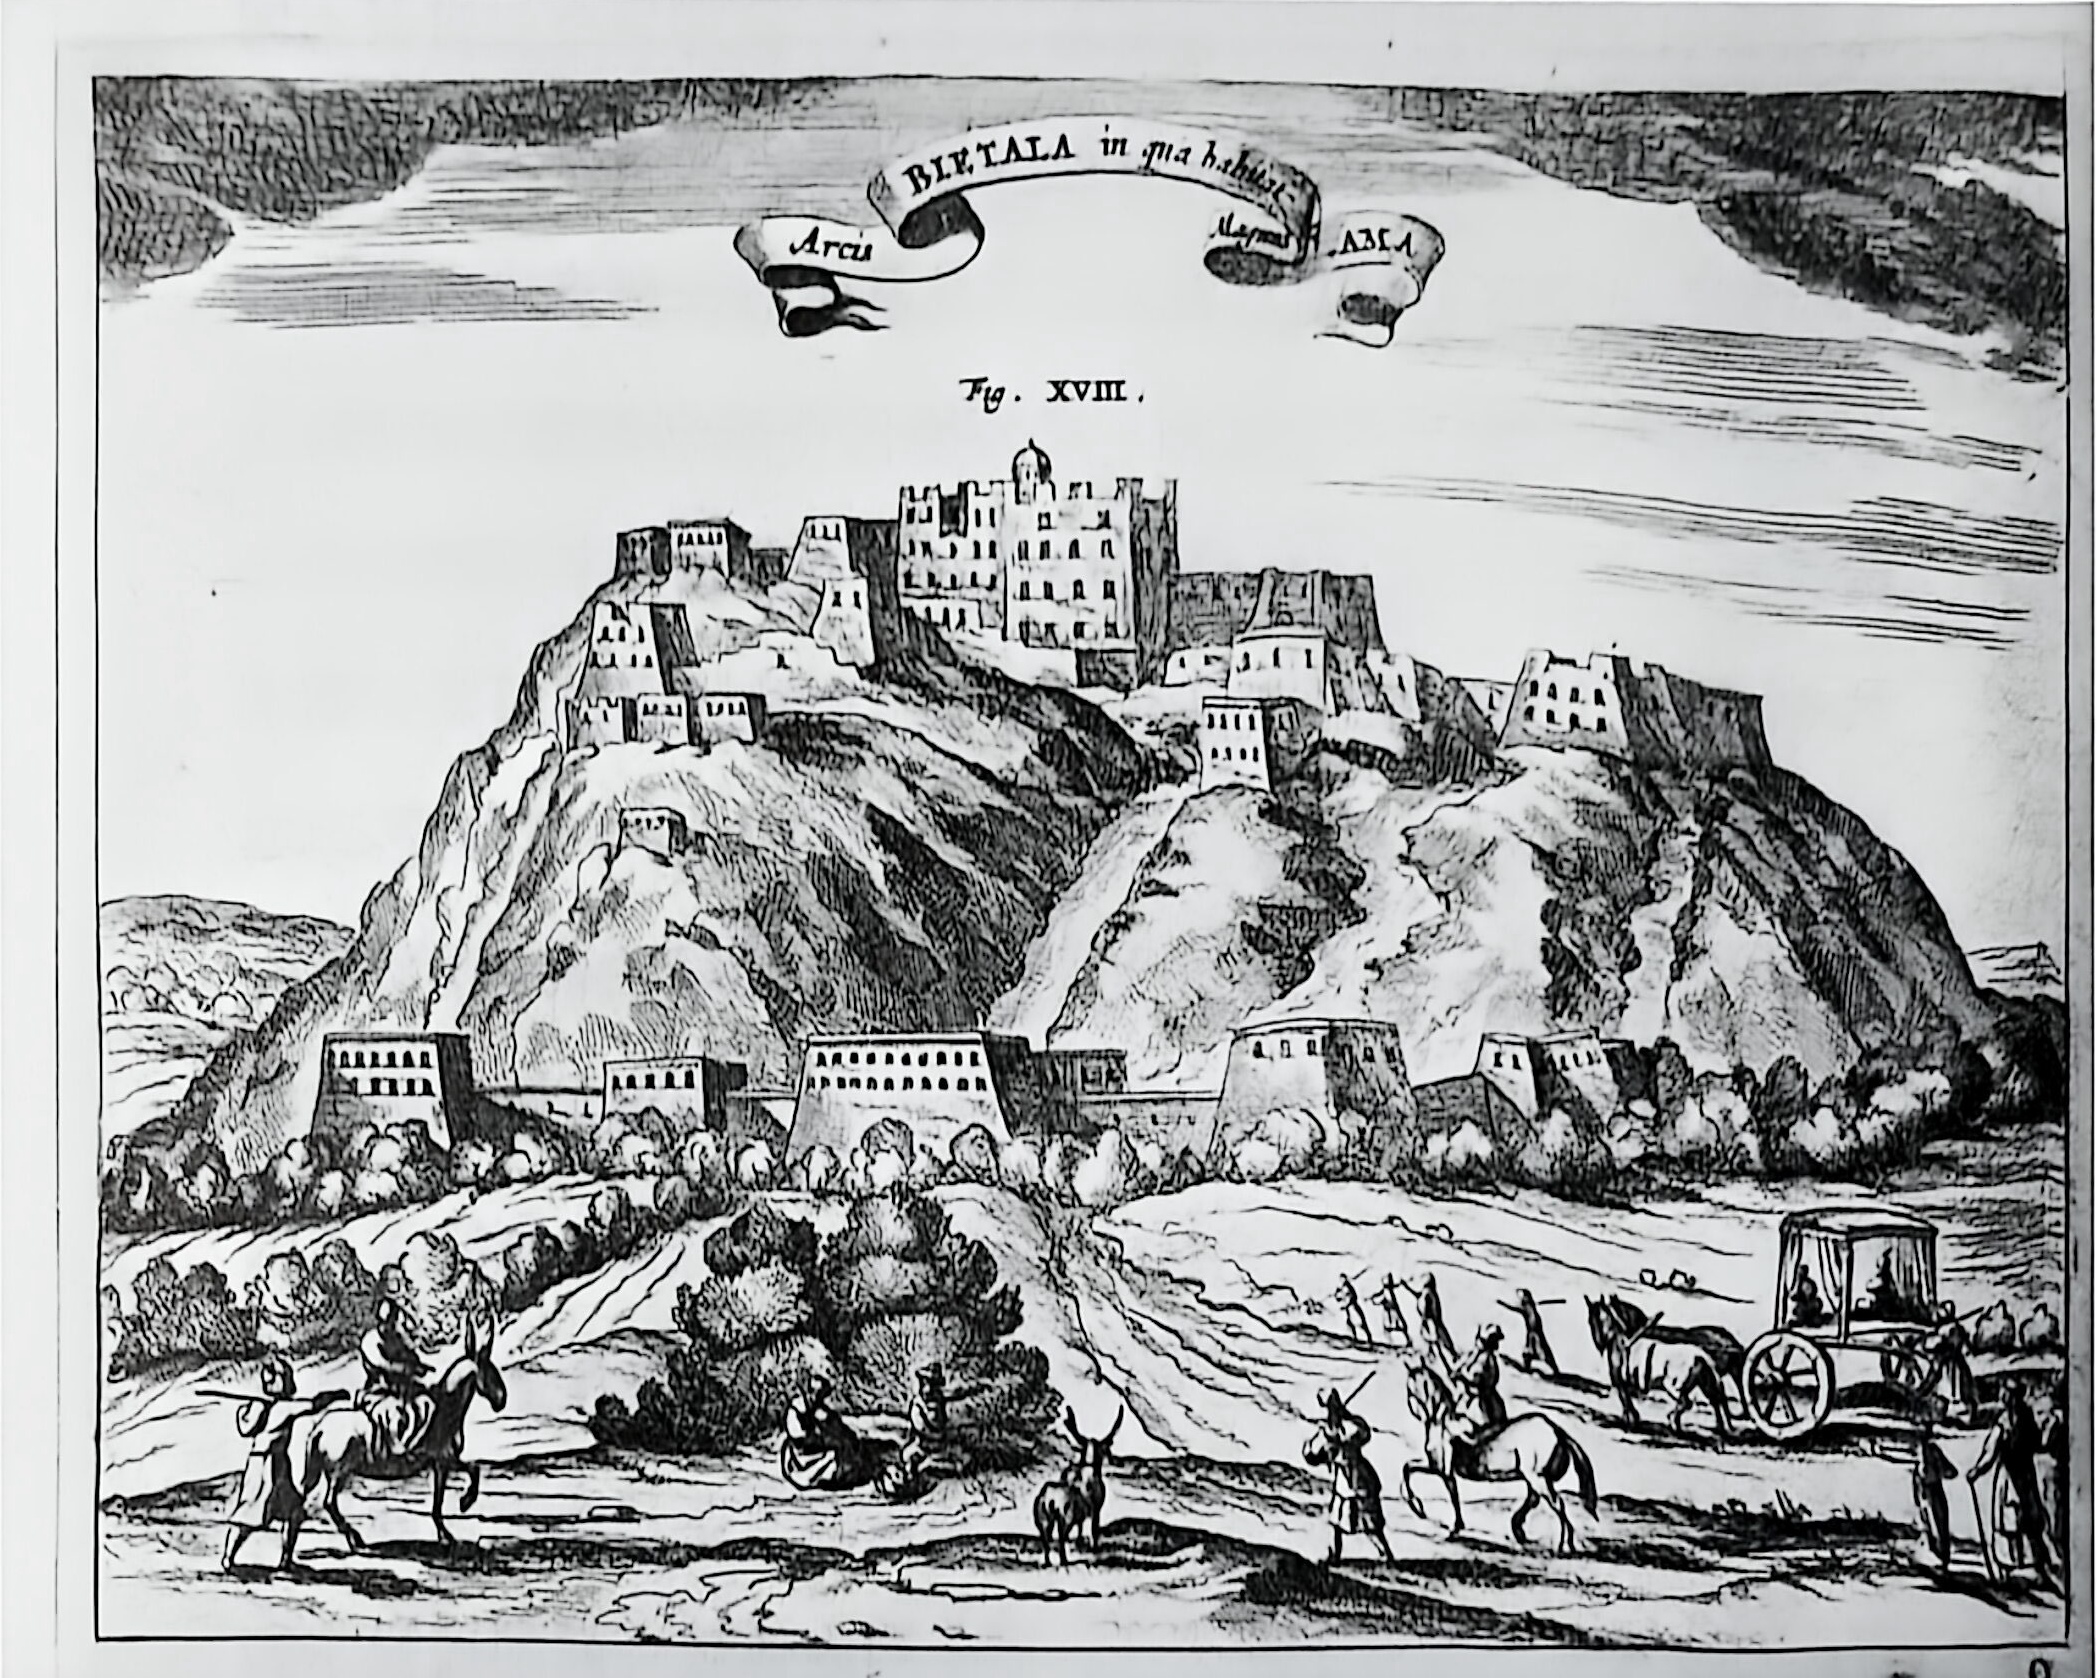
\includegraphics[width=.9\linewidth,height=.68\textheight,keepaspectratio]{assets/fig-298.jpg}
\caption{布达拉宫全景图，Athanasius Kircher, China Illustrata, 1667 (Division of Rare and Manuscript Collections, Cornell University Library)}\label{fig:298}\end{figure}


% 原书第278–279页

过去的康熙储位问题研究，都发现康熙从五十六年底开始的立太子讨论，在五十七年初突然中止了。其实，这并不是康熙对立太子问题有了新想法，而是因为他被突发的准噶尔和西藏问题搅乱了心神，集中精力去应战了。康熙对西线用兵的安排，现在用文字写出来就是几段话，但当时要在青海、甘肃、新疆、西藏这些地方调度人力、军力、粮草事务，样样都是大工程，而且还要从各方面收集并甄别信息。我们现在回顾历史，一目了然，事态如何一步一步发展都看得清清楚楚。但当时的康熙和前方将领却是在猜测中行动。\NoteRef{07}{30}根据传教士的记录，他们赶路的速度，从西安到西宁需要二十三天，从西宁到拉萨需要八十天。\NoteRef{07}{31}当时西宁以外并无驿站。许多拉萨发生的事，传到北京都有三个月左右的延后。最早康熙知道准噶尔兵进藏，却不清楚这支军队进藏的目的。因为拉萨的拉藏汗与策妄阿喇布坦之前有姻亲关系，康熙甚至怀疑这支军队是去帮助拉藏汗做某些事情的。\NoteRef{07}{32}到后来，西藏已然陷落，康熙却还不确定准噶尔军队到底有多少人在拉萨。康熙和朝廷迅速切换到了战争准备模式。这才是康熙突然中止太子问题讨论的一个现实原因。


% 原书第279–280页

整个1718年最让康熙不能接受的是，在朝廷忙了大半年，等来的却是七千兵马在西藏完败的消息。\NoteRef{07}{33}这对康熙和整个清廷来说都是奇耻大辱。草原民族最重名誉，而名誉是靠一场一场战争打出来的。这份名誉让康熙说话有分量，具有维护地区和平的震慑力。清朝疆域辽阔，不同地区的大小部落，民族不同，信仰不同，不可能一个一个管理，而要依靠震慑力使这些地方主动臣服。现存的清史资料对于这次惨败的奏报和记录都比较简短，是在有意淡化。但是当时清军大败的消息迅速传遍了蒙古和中亚地区，身处拉萨的嘉布遣会神父在1719年2月的一封信中，也把消息发回了欧洲。\NoteRef{07}{34}为了稳定军心，也为了顾全颜面，康熙没有在朝廷公布两支入藏军队全军覆灭的消息。总督额伦特去世的消息连他的亲弟弟都没有告知。1719年夏，也就是康熙得知额伦特阵亡半年后，收到了额伦特弟弟写来的密折，称从嫂子的来信得知他的哥哥已于去年秋天阵亡，问康熙为什么自己没有得到通知，死讯也没有宣布。康熙答复说，请他为国再坚持一段时间，保守秘密：


% 原书第280页

\begin{bookquote}暂且隐忍等候为妥。西宁大将军王亲往祭奠尔兄之遗体，此等情由，朕本应降旨，令尔知晓。因有军机事务，尚未晓谕于尔，事成之后，再降谕旨。尔兄英勇效力，全国追念，如鲠在喉，朕书此数言，潸然泪下！\NoteRef{07}{35}\end{bookquote}

% 原书第280页

额伦特此前是湖广总督，乃清朝最高级别的地方官，同时也是跟随康熙几十年的老臣子。所以对于康熙来说，额伦特战死沙场，于公于私都是令人心痛的事。清朝的前方将士一直在收集这两支部队如何失败的相关信息。在回复这份奏折前大概一个多月，康熙五十八年四月初三日（1719年5月21日），康熙让皇十四子举行了仪式祭奠额伦特及阵亡士兵，并请喇嘛诵经。\NoteRef{07}{36}同时，康熙通过多个渠道数次发文给准噶尔一方，要求他们送回侍卫色楞。\NoteRef{07}{37}


% 原书第280–281页

北京获得两支军队兵败的消息是在康熙五十七年九月二十九日（1718年11月21日）。而在接到他们战败消息前十天，康熙还满怀希望，给年羹尧等靠近藏区的地方官员颁发满文上谕，让他们想办法通过入藏人员给藏地喇嘛带话带文，表示康熙才是真正的“佛教大施主”，并告知众人清军正在赶来，劝他们不要投靠新的政权。因此可以想见，康熙突然收到全军覆灭的消息后该有多么震惊。\NoteRef{07}{38}


% 原书第281–282页

在康熙眼中，整个从1715年开始于哈密的摩擦都是由策妄阿喇布坦挑起的。康熙曾通过西北的部落给策妄阿喇布坦发过公开信：“兹太平安谧之际，谁无故滋事，扰害众生，谁则咎由自取，此事尔很明白。”\NoteRef{07}{39}康熙勒令他息兵，以免生灵涂炭。\NoteRef{07}{40}但策妄阿喇布坦不仅没有听从康熙的警告，紧接着又侵犯了拉萨，歼灭了清军，完全没有把康熙的话放在心里。从五十六年（1717）夏得知准噶尔兵入藏，到五十七年（1718）初听闻拉萨陷落，再到年底获悉军队被全歼，康熙运筹帷幄一年半后，等来了超乎他预期的最坏结果。一是出兵被全歼，完全出乎意料，以致他“心情郁闷”。\NoteRef{07}{41}第二，他之前信誓旦旦对朝廷众人讲话，显示出一切尽在掌握的必胜姿态，可突然传来的失败让他颜面尽失。这也是他没有公布额伦特去世消息的原因。后来他甚至要求前方不要频繁递送消息，以免引起朝廷众人“胡乱猜疑”。\NoteRef{07}{42}第三，藏传佛教对康熙来说还有宗教上的情感，因此拉萨是他从来没有想到会失去的地方。尽管康熙没有公开表明过自己的信仰，但从他遇到困难时选择念诵藏文佛经，就知道他在宗教层面是倾向于藏传佛教的。而且早在二十年前征讨准噶尔时，康熙就被蒙藏各部称为文殊菩萨。\NoteRef{07}{43}蒙藏地方头目给康熙的信函都是如此开头：“谨自远方合掌跪奏天地间，以威福统驭万方，文殊师利皇帝洁如莲花宝座前”，“谨奏深居大国正中之文殊师利之呼毕勒罕（呼毕勒罕是蒙语中的转世之人），以统御环宇之君主容貌，扶佑天下一切，无以伦比之仁主明下。”\NoteRef{07}{44}这次西藏被灭时统治西藏的拉藏汗，给康熙上书，用词是这样的：


% 原书第282页

\begin{bookquote}无知小人我向度量谋略超卓之文殊师利皇帝启奏虽难，但倚前世恩缘，以如雨滴益于海之清白之心具奏，若有非是，请予鉴谅。\NoteRef{07}{45}\end{bookquote}

% 原书第282页

除了周边的蒙藏头目这样称呼康熙，遥远的车臣汗部首领给康熙的书函也称其为文殊皇帝。\NoteRef{07}{46}对康熙以及所有信仰藏传佛教的蒙藏各部来说，拉萨都是他们的圣地。这其中的宗教情结在康熙发到蒙藏各部以及给策妄阿喇布坦的信中，多有体现：他以“大施主”自居，给策妄阿喇布坦定的罪是“毁坏我等共奉之法度”，而兴兵的理由是：“为振兴佛法，遣众施主前往。”\NoteRef{07}{47}此外，“满洲”这个名称的来源就一直传言和文殊菩萨有关——文殊菩萨梵文读音用字母转写后是Maňjuśrī。\NoteRef{07}{48}


% 原书第282–283页

在得知战败消息后，无论于公，于私，于世俗公道，于国家战略，于个人颜面，康熙都必须亮明态度。于是，他迫不及待地任命了一位抚远大将军，总领西北各路兵马，决心夺回拉萨，重振清军威名。任命这一天是康熙五十七年十月十二日（1718年12月3日），距离得知战败消息的九月二十九日（1718年11月21日），仅过了十二天。得到这个大将军职位的，正是皇十四子。


% 原书第283页

十二月十二日（1719年1月31日），康熙给皇十四子安排了规模空前的出征仪式：


% 原书第283页

\begin{bookquote}上命内阁大臣颁给大将军敕印于太和殿。其出征之王、贝子、公等以下悉戎服侍太和殿前，其在京王、贝勒、贝子、公并二品以上大臣等，悉蟒服侍午门外。允禵（注：皇十四子）上殿跪受敕印，谢恩，行礼，出。诸王以下，二品大臣以上，随至列兵处。允禵望阙，叩首，肃队而行。\NoteRef{07}{49}\end{bookquote}

% 原书第283–284页

王锺翰评论：“其庄严隆重若此，清初以来所未有也。”\NoteRef{07}{50}皇十四子后来进藏时指挥的军队号称是三十万人。\NoteRef{07}{51}从出兵仪式之盛大，到统帅军队的规模，都可以看出皇十四子这次本质上就是代康熙出征。其实，早在1717年康熙得知策妄阿喇布坦又在向西藏派兵时，他就在与前线将领的通信中表示过，要不是他已经上了年纪，早已御驾亲征了：


% 原书第284页

\begin{bookquote}朕年日增，血气渐衰，故此事迟疑至今。如当朕少壮时，早已成功矣。\NoteRef{07}{52}\end{bookquote}

% 原书第284页

康熙多次展露出“封狼居胥，燕然勒石”这种汉代武将的情怀，也早就有心派出一位能够直接统帅各路人马的将领。他一直没有采取大的行动，很大原因是被传来的各种不知真假的信息误导了，再加上之前1715年的哈密危机，他已经派出了吏部尚书，本以为会大打一仗，结果前方传回来的消息却是两百清军就化解了危机。康熙虽然没有大的调动，但是一直在做准备。比如他往成都和西安调兵：“顾念地方遥远，消息到后方调兵则不及。”\NoteRef{07}{53}所以，尽管从1716到1718这三年康熙没有大的动作，但他应设想过真要到了用兵那一天，该推出来的人选。皇十四子在十多天内被选中，并不是康熙的一时兴起，而是深思熟虑后的结果。


% 原书第284页

在宣布皇十四子为抚远大将军之后八天，康熙给出了第二项西征的重大任命：把年羹尧从四川巡抚升为四川总督。这样他可以全权负责四川的民事和军务。在颁布这项任命的同时，康熙还对年羹尧之前在四川的表现给予了高度的肯定，赞扬他：“自军兴以来办事明敏。”\NoteRef{07}{54}


\begin{sectionnotes}

% 原书注释：原书第422页
\BookNote{07}{1}{最早研究清朝与西藏关系的是Luciano Petech, China and Tibet in the Early 18th Century: History of Establishment of Chinese Protectorate inTibet。该1950 年代出版的研究主要使用的是藏族档案材料外加清朝官方史书，至今仍然是领域中的经典。1980年代以来清宫档案、奏折陆续出版后，平定西藏新近研究的代表作品：柳陞祺，《十八世纪初清政府平定西藏准噶尔之乱始末》；邓锐龄，《1720年率军进入拉萨的清军将领——延信》（初刊于1999年），《1720年清军进入西藏的经过》（初刊于2000年），《年羹尧在雍正朝初期治藏政策孕育过程中的作用》（初刊于2002年）以及 Peter Perdue, China Marches West: The Qing Conquest of Central Eurasia。以上为清军入藏路线及整体性研究。另外，皇十四子和年羹尧与入藏的相关问题还出现在涉及康熙朝储位之争的诸多研究中。限于篇幅，在此不一一列举。}

% 原书注释：原书第423页
\BookNote{07}{2}{若松宽，《策妄阿喇布坦的崛起》。}

% 原书注释：原书第423页
\BookNote{07}{3}{张建，《再造强权—准噶尔珲台吉策妄阿喇布坦崛起史新探》。}

% 原书注释：原书第423页
\BookNote{07}{4}{《圣祖仁皇帝亲征平定朔漠方略》，《景印文渊阁四库全书》，卷28，三十五年八月甲午。}

% 原书注释：原书第423页
\BookNote{07}{5}{若松宽，《策妄阿喇布坦的崛起》，96—99。}

% 原书注释：原书第423页
\BookNote{07}{6}{康熙与策妄阿喇布坦早年互相配合攻打噶尔丹，见《康熙朝满文朱批奏折全译》，169。}

% 原书注释：原书第423页
\BookNote{07}{7}{《平定准噶尔方略》，前编卷01，康熙五十四年四月甲午。}

% 原书注释：原书第423页
\BookNote{07}{8}{《平定准噶尔方略》，前编卷01，康熙五十四年四月甲申。}

% 原书注释：原书第423页
\BookNote{07}{9}{若松宽，《策妄阿喇布坦的崛起》。}

% 原书注释：原书第423页
\BookNote{07}{10}{赵柄学，《策妄阿拉布坦和清朝关系史之研究—从〈清内阁蒙古堂档〉研究18世纪清朝和准噶尔蒙古关系》。}

% 原书注释：原书第423页
\BookNote{07}{11}{Lisa Hellman, "Enslaved in Dzungaria: What an Eighteenth-Century Crocheting Instructor Can Teach Us about Overland Globalization", 380, note 48. Pär Cassel, “Solitary Swedish Sinologists: Three Hundred and Fifty Years of Swedish China Studies", 466.}

% 原书注释：原书第423页
\BookNote{07}{12}{Lisa Hellman, “Enslaved in Dzungaria: What an Eighteenth-Century Crocheting Instructor Can Teach Us about Overland Globalization", no.3,380.}

% 原书注释：原书第423页
\BookNote{07}{13}{Lisa Hellman, "Enslaved in Dzungaria: What an Eighteenth-Century Crocheting Instructor Can Teach Us about Overland Globalization", 379.}

% 原书注释：原书第424页
\BookNote{07}{14}{Nicholas Poppe, “Renat's Kalmuck Maps", 157-159.}

% 原书注释：原书第424页
\BookNote{07}{15}{宋嗣喜，《策妄阿喇布坦与沙皇俄国博罗库尔干出使俄国、温科夫斯基出使准噶尔与达尔扎复又出使俄国评述》。}

% 原书注释：原书第424页
\BookNote{07}{16}{《平定准噶尔方略》，前编卷04，康熙五十六年八月壬午。}

% 原书注释：原书第424页
\BookNote{07}{17}{《平定准噶尔方略》，前编卷04，康熙五十六年八月丁未。}

% 原书注释：原书第424页
\BookNote{07}{18}{《平定准噶尔方略》，前编卷04，康熙五十六年十月乙巳，罗卜藏丹津奏报及议政大臣会议分析，见《康熙朝满文朱批奏折全译》，1257—1260。}

% 原书注释：原书第424页
\BookNote{07}{19}{《平定准噶尔方略》，前编卷04，康熙五十六年十一月甲戌。}

% 原书注释：原书第424页
\BookNote{07}{20}{《平定准噶尔方略》，前编卷04，康熙五十六年七月辛未。}

% 原书注释：原书第424页
\BookNote{07}{21}{《平定准噶尔方略》，前编卷04，康熙五十七年二月庚寅。}

% 原书注释：原书第424页
\BookNote{07}{22}{这一占领时期拉萨的详细情况，参看Luciano Petech，China and Tibet in the Early 18th Century: History of Establishment of Chinese Protectorate in Tibet, 25–54。}

% 原书注释：原书第424页
\BookNote{07}{23}{当时拉萨有四位神父。在准噶尔士兵入城时，有两位在城外，得幸免。在城内的两位遭遇了殴打和抢劫。被殴打神父写出的亲身经历，见I Missionari Italiani nel Tibet e nel Nepal, v.1, 109–110；详细内容参看Vannini, The Bell of Lhasa, 191-192；德西德里当时不在拉萨城内，但他记录了方济嘉布遣会神父的遭遇。Desideri,An Account of Tibet, 157–158.}

% 原书注释：原书第424页
\BookNote{07}{24}{Yuval Givon, “Connecting Eurasia: Jesuit Experimentation with Overland Mobility Between China and Europe, 1656-1664", 647- 649.}

% 原书注释：原书第425页
\BookNote{07}{25}{拉萨在准噶尔进入前的情况，参看Michael J. Sweet and Leonard Zwilling, "The First Capuchin Mission to Tibet: Fr. Domenico da Fano's Report of 1713”；关于方济嘉布遣会神父入藏经历，以及西安神父的报告，见I Missionari Italiant nel Tibet e nel Nepal, v.1, 63-66；教皇给拉藏汗的信，见I Missionari Italiani nel Tibet e nel Nepal, v.4, 175。}

% 原书注释：原书第425页
\BookNote{07}{26}{《平定准噶尔方略》，前编卷05，康熙五十七年六月壬午。}

% 原书注释：原书第425页
\BookNote{07}{27}{《平定准噶尔方略》，前编卷05，康熙五十七年闰八月丁未。}

% 原书注释：原书第425页
\BookNote{07}{28}{从最后额伦特发回的奏报看，两位统帅对于扎营位置的选取有不同意见，可能是大败的一个原因。《平定准噶尔方略》，前编卷05，康熙五十七年九月甲辰；《康熙朝满文朱批奏折全译》（页1394）中可以看到后来在询问幸存官兵“额伦特、色稜（楞）不睦之缘由”；另外康熙的一封谕旨中也提到二人不和，《康熙朝满文朱批奏折全译》，页1442；Petech通过藏文资料也认为失败与二人意见不合有关。Luciano Petech, China and Tibet in the Early 18th Century: History of Establishment of Chinese Protectorate in Tibet,67.}

% 原书注释：原书第425页
\BookNote{07}{29}{清廷一直在前方打探两支军队的消息。后来有两军残部返回，详细讲述了当时的战斗情况。《康熙朝满文朱批奏折全译》，1392一1394。}

% 原书注释：原书第425页
\BookNote{07}{30}{现存康熙朝满文奏折中有一份很长的（约七千五百字）综合各方面信息的前线分析。从分析中可以看出，康熙与朝臣对很多信息都无法判定真假，比如对准噶尔入藏军队的大概规模就无从得知。《康熙朝满文朱批奏折全译》，1228—1232。}

% 原书注释：原书第426页
\BookNote{07}{31}{I Missionari Italiani nel Tibet e nel Nepal, v.1, 65.}

% 原书注释：原书第426页
\BookNote{07}{32}{白新良，《康熙后期经营西疆失载年月满文档案考辨》，《清史考辨》（2006），265。拉藏汗与策妄阿喇布坦之间“每年彼此有往来”，见《元以来西藏地方与中央政府关系档案史料汇编》，第2册，311；康熙甚至怀疑二人在合谋想要夺取其他地方，见《元以来西藏地方与中央政府关系档案史料汇编》，第2册，315。关于传教士记载往来西安到拉萨的时间，见I Missionari Italiani nel Tibet e nel Nepal, v.1, 65–66。}

% 原书注释：原书第426页
\BookNote{07}{33}{七千是传教士留下的数字。Luciano Petech, China and Tibet in the Early I8th Century: History of Establishment of Chinese Protectorate inTibet,56.现在确知是色楞带兵两千多人在前，但总督额伦特带了多少兵尚未发现准确记录，这个问题学界尚有争议，因为后来康熙公开说，清军两支部队总共只有三千多人。《平定准噶尔方略》康熙五十七年三月有额伦特建议如何用兵的奏折，当时提到了色楞有二千四百多兵马，同时他说色楞兵马太少。他提到他自己手下也有两千兵。同时他还建议从别处征调兵丁，由他率领。额伦特出兵时原计划是单独一路进攻拉萨，只是后来色楞求援，才与其汇合。从他原计划是单独一路兵马这个角度来说，他带的兵不会少于色楞。所以传教士所说的七千人总数是有可能的。}

% 原书注释：原书第426页
\BookNote{07}{34}{Luciano Petech, China and Tibet in the Early 18th Centuoy: History of Esta- blishment of Chinese Protectorate in Tibet, 56, note 1.}

% 原书注释：原书第427页
\BookNote{07}{35}{《康熙朝满文朱批奏折全译》，1399—1400。}

% 原书注释：原书第427页
\BookNote{07}{36}{《康熙朝满文朱批奏折全译》，1390。在这之前，皇十四子已经从多个途径收集到了额伦特部队的情况。有一些幸存士兵从不同途径逃回了内地。跟额伦特交战的就是准噶尔主力，但准噶尔主将得知额伦特阵亡后，主动表示停战，同时带话给清军表示他本无意斩杀清军主将，清军可以带着主将尸体撤离，这也是额伦特尸骨能够带回的原因。后来清朝收复西藏后，一直和准噶尔在和谈，就是因为双方在战争中并没有引起太多的仇恨。包括被准噶尔俘获的400多清军，并没有遭到斩杀，而是囚禁一段时间后，在班禅喇嘛的协调下，全部放还，班禅喇嘛还以私人名义给了这些士兵衣物盘缠。据返归士兵称，当地藏民对待内地人友善，悄悄给与他们食物。《康熙朝满文朱批奏折全译》，1392一1394。}

% 原书注释：原书第427页
\BookNote{07}{37}{《康熙朝满文朱批奏折全译》，1530。}

% 原书注释：原书第427页
\BookNote{07}{38}{《康熙朝满文朱批奏折全译》，1330。}

% 原书注释：原书第427页
\BookNote{07}{39}{《康熙朝满文朱批奏折全译》，1530。}

% 原书注释：原书第427页
\BookNote{07}{40}{《平定准噶尔方略》，前编卷01，康熙五十四年四月甲申。}

% 原书注释：原书第427页
\BookNote{07}{41}{康熙在得知兵败五天后，在闽浙总督满保所上的请安折中批道：“朕体安善。今年比往年好，唯心情郁闷……”他没有告诉满保是什么事情。《康熙朝满文朱批奏折全译》，1334。}

% 原书注释：原书第427页
\BookNote{07}{42}{“频繁具奏，有劳驿站，且京城之人不知何事，不能停止其胡乱猜疑。”《康熙朝满文朱批奏折全译》，1369。}

% 原书注释：原书第427页
\BookNote{07}{43}{比如《康熙朝满文朱批奏折全译》，136，143，181。}

% 原书注释：原书第427页
\BookNote{07}{44}{《康熙朝满文朱批奏折全译》，143，168，169，252。}

% 原书注释：原书第428页
\BookNote{07}{45}{《康熙朝满文朱批奏折全译》，399。}

% 原书注释：原书第428页
\BookNote{07}{46}{《康熙朝满文朱批奏折全译》，1675。}

% 原书注释：原书第428页
\BookNote{07}{47}{《康熙朝满文朱批奏折全译》，1527。}

% 原书注释：原书第428页
\BookNote{07}{48}{相关考证有很多，比如王俊中，《“满洲”与“文殊”的渊源及西藏政教思想中的领袖与佛菩萨》，89—132。}

% 原书注释：原书第428页
\BookNote{07}{49}{《平定准噶尔方略》，前编卷05，康熙五十七年十二月乙卯。}

% 原书注释：原书第428页
\BookNote{07}{50}{王锺翰，《胤祯西征纪实》，《王锺翰清史论集》，1119。}

% 原书注释：原书第428页
\BookNote{07}{51}{Peter Perdue, China Marches West: The Qing Conquest of Central Eurasia,235. 实际投入军队数小于10万人。}

% 原书注释：原书第428页
\BookNote{07}{52}{《平定准噶尔方略》，前编卷04，五十六年七月辛未。}

% 原书注释：原书第428页
\BookNote{07}{53}{《康熙朝满文朱批奏折全译》，1232。}

% 原书注释：原书第428页
\BookNote{07}{54}{《平定准噶尔方略》，前编卷05，康熙五十七年十月甲子。}

\end{sectionnotes}
\section{康熙栽培的年羹尧}

% 原书第285页

说到年羹尧（1679—1726），无论是学术研究还是小说电视，都会首先把他联系到雍正，说他是雍正的藩邸旧人，认为他的仕途兴起得益于雍正。但实际上年羹尧的仕途与雍正的联系很少，他其实是康熙一手栽培、提拔的封疆大吏，是康熙十分欣赏的文武全才。从1700年中进士，到1726年初被雍正赐死，年羹尧混迹官场的二十六年中，除去下狱后审讯的时间，真正在雍正手下做事不到三年。在最后给雍正上的奏折中，年羹尧写道：


% 原书第285页

\begin{bookquote}若是主子天恩怜臣悔罪，求主子饶了臣，臣年纪不老，留下这一个犬马慢慢的给主子效力。……伏地哀鸣，望主子施恩，臣实不胜呜咽。\NoteRef{07}{55}\end{bookquote}

% 原书第285页

臣年纪不老”，被雍正赐死时，年羹尧仅四十八岁。这封求生奏折的行文语气和前面章节提到过的皇三子自称奴才给雍正上的密折十分相似。而年羹尧的这份奏折也就比皇三子所写早几个月时间。他和皇三子一样，都曾经是康熙极为欣赏、倚重的实力派人物。而这般低声下气地上奏折，则是年羹尧在康熙朝没有过的。


% 原书第286页

年羹尧是康熙三十九年庚辰科（1700）进士，是不折不扣的文臣出身。\NoteRef{07}{56}他获取进士时仅二十二岁，加上他属于镶白旗下的汉军旗人，一进入官场就是各方争抢的对象——这年共有三百零五位进士，其中只有十五位八旗子弟。\NoteRef{07}{57}康熙把年羹尧选入了翰林院，明珠又把他的孙女，也就是纳兰性德的女儿，许配给了年羹尧。纳兰性德早亡，对亲事做主的应该正是明珠。纳兰世家隶属于正黄旗，家世显赫，与身世普通的年家并非门当户对。能结成这门亲事，应该是明珠相中了年羹尧的才华。1706年，明珠第三子纳兰揆方的夫人去世，邀请年羹尧为墓志铭撰文，同时请王鸿绪为墓志铭篆盖。\NoteRef{07}{58}能被邀请为明珠儿媳的墓志铭撰文，是当时权贵圈对年羹尧文才认可的标志。这一时期的年羹尧，与王鸿绪等人在京城有着相仿的身份标识。


% 原书第286–287页

从1700年到1709年的九年时间里，年羹尧都供职于翰林院。这一时期最能代表其文臣形象的是他被朝廷委派去四川（1705）和广州（1708）两地做乡试的主考官。\NoteRef{07}{59}这是进士进入翰林院后，学问获得认可的一个标志。同时，这一时期他做过翰林院侍读和侍讲，这两个职位让他接触到了康熙，使康熙对他有了直接了解。\NoteRef{07}{60}1709年春，在复立太子前，年羹尧被授予了内阁学士兼礼部侍郎之职。\NoteRef{07}{61}内阁学士只有十个名额，是所有翰林院官员梦寐以求的职位。获取这个职位表示得到了皇帝的认可，有资格帮助皇帝处理朝廷系统传递上来的公文。\NoteRef{07}{62}前文讲过，复立太子前，康熙与群臣对立。年羹尧在这一时期突然得到提拔，很可能是他在太子废立问题上的表现，符合康熙的期许，得到了康熙的信任。在正式复立太子后，年羹尧被派以副使身份（正使是康熙的一个侍卫）到朝鲜宣布太子复立事宜。\NoteRef{07}{63}年羹尧被委派处理太子相关的问题，表明这时康熙已经把他当作了自己人（参看书签二时间表）。


% 原书第287页

从朝鲜返回后，1709年秋，康熙委任年羹尧为四川巡抚。在年羹尧外放之时，康熙对他寄予厚望，给他讲：


% 原书第287页

\begin{bookquote}比年湖广百姓，多往四川开垦居住，地方渐以殷实。为巡抚者，若一到任即欲清丈地亩、增加钱粮，即不得民心矣。湖南因丈量地亩，反致生事扰民。当年四川巡抚噶尔图曾奏请清丈，亦未曾清楚。尔须使百姓相安，钱粮以渐次清查可也。此为四川第一要事。\end{bookquote}

% 原书第287页

康熙对年羹尧的关爱，从他出去上任时就已经显露出来。康熙预计此时三十出头的年羹尧会像传统的文官一样，到了地方为求政绩，会从收税入手。康熙深知这会带来麻烦，提醒他去了先别做这件事。康熙还告诉第一次出去做官的年羹尧：


% 原书第288页

\begin{bookquote}地方武官每获一小贼辄张大声势，自以为大有劳绩。盗贼何处无有？但须严行巡缉，不可将小事看大了。武官当勿令生事，然亦须稍留余地，使伊等养给其家。尔为巡抚，须文武和衷，不可偏刻。\NoteRef{07}{64}\end{bookquote}

% 原书第288页

然亦须稍留余地，使伊等养给其家”，这是康熙版本的“水至清则无鱼，人至察则无徒”。康熙能把这样的治理地方的切实经验告诉年羹尧，显然是把他当成了自己人。康熙给年羹尧最大的照顾，也可以说是特权，就是允许他密折汇报。正常情况下，地方官员向中央奏请，无论大小事宜都是走朝廷公家渠道。有资格用密折汇报的只有部分康熙亲近的在地方上的包衣奴才，或者是像王鸿绪那样的特许之人。年羹尧在其离京时就得到了这项特权。


% 原书第288页

年羹尧被外派四川的这年冬天（康熙四十八年，1709年），还有一件影响他最终命运的事发生。康熙册封了皇三子、皇四子、皇五子、皇七子和皇十子五位皇子为王。皇四子被封为和硕雍亲王。\NoteRef{07}{65}这次封王本来和年羹尧没有任何关系，但封王意味着八旗内人事财产的分配。年羹尧家隶属的镶白旗汉军旗牛录（八旗中的基本行政单位）被划到雍亲王名下。这样一来，雍亲王便成为了年家上下的主子，雍亲王与年羹尧建立了主属关系。\NoteRef{07}{66}


% 原书第289页

如果抛开后见之明，在不知道雍亲王后来会成为皇帝的情况下，切实站在年羹尧的角度来思考这次分封，就会发现年羹尧其实不会觉得这次分封能对自己造成什么影响。他与雍亲王的关系就是名义上的。当时已经做到内阁学士和四川巡抚的年羹尧，之前的仕途完全是他自己走出来的，跟雍亲王没有丝毫关系；同时，他已经做到这个职位，又深得康熙信任，个人未来的仕途也完全取决于康熙。所以尽管年家的主属关系转到了雍亲王处，但年羹尧没有主观动机去亲近他的这个新主子。这一点是理解康熙最后十三年里年羹尧与雍亲王关系的关键。


% 原书第289页

年羹尧于康熙四十八年十二月十五日（1710年1月14日）到成都上任，两个月后，他就给康熙上了一份约两千字的长折，条陈四川“积弊”，并给出了他的整改意见。这份长折的核心内容是关于四川官员贪腐的问题。在奏折的最后，他点名向康熙报告：


% 原书第289页

\begin{bookquote}至通省官员，臣虽未曾尽见，而查阅旧案，细访民情，止有提学道陈瑸一人考试公明，一尘不染，将来自是为皇上出力之人。布政司卞永式贪劣无能（朱批旁批：一点不错），臣以到任不久，未得确实款迹，伏乞皇上特旨革斥，以张乾断不测，则通省官吏咸畏法知警矣。\end{bookquote}

% 原书第289–290页

\begin{bookquote}缘系密奏折子，臣自缮写，不敢使一人得知，谨遣家人魏之耀赍奏。其字画潦草，文理疏谬，伏乞皇上格外恕臣。\NoteRef{07}{67}\end{bookquote}

% 原书第290页

年羹尧一到地方就敢于对当地官员做出这样直言不讳的评判，并密折发给康熙，这说明年羹尧知道康熙信任他的判断。而这时年羹尧还是文臣，奏折的最后还在担心“字画潦草，文理疏谬”。


% 原书第290页

在上了这封奏折不久，康熙四十九年（1710）夏，四川西南的建昌（今西昌一带）“番蛮”杀死了一位朝廷官员。朝廷派年羹尧前去调查。本来这个案件涉及了兵事，不归掌管民事的巡抚负责，但正巧这一时期分管军事的四川提督岳昇龙患有眼疾。岳昇龙在前章提到过，早在征讨三藩时就已是著名武将，后来又跟随康熙亲征过噶尔丹，在太子被废期间还给康熙上过奏折表示遗憾。简单来说，这位久经沙场的老将是康熙的老相识。但岳昇龙一直没有因为患了重病而向康熙和朝廷提起辞呈。康熙应该从其他渠道得知了岳昇龙患病之事，所以才派年羹尧前往处理。这是年羹尧身为文臣而料理军务的开始。


% 原书第290页

康熙还私下让年羹尧去切实调查岳昇龙的病情。岳昇龙1690年代就入川掌兵，熟悉四川边地。年羹尧入川后，岳昇龙应该对年羹尧也多有照顾。年羹尧在康熙面前高度赞扬岳昇龙，说：


% 原书第291页

\begin{bookquote}……提臣久任川省，熟悉边疆，即臣之得知羌蛮情形，皆平日闻之提臣所说，此实武臣中之深晓边情者。\NoteRef{07}{68}\end{bookquote}

% 原书第291页

年羹尧和岳昇龙有交往，他也不愿意私下向康熙报告岳昇龙的病情。因而当康熙问到他时，他在汇报岳昇龙“两目病废”时，特意强调岳昇龙亲口告知他，自己已经向朝廷如实禀报了病情，所以他就没有私下向康熙禀奏。康熙收到年羹尧汇报病情的密折后，马上告知年羹尧切莫让人知道他追查过病情。康熙用朱笔写道：


% 原书第291页

\begin{bookquote}提督久任封疆，名望甚大，可惜两目失明，已难做官。但本人不曾具题，等他具题时，自有温旨。此折断不可令人知道。\NoteRef{07}{69}\end{bookquote}

% 原书第291–292页

康熙让年羹尧配合装作不知道岳的病情，意在保全岳的面子，等他自己呈报。康熙与年羹尧这样一来一回的交流，充分显示了他对年羹尧的信任，同时也在教年羹尧如何平衡公私人情。后来，岳昇龙辞了官，年羹尧才向康熙禀报了岳昇龙早就身体不殆，却迟迟未提辞呈的原因。原来岳昇龙从1702年开始，和其他一些官员动用了公款，欠库银三万九千二百八十两。在奏折中，年羹尧同时提出了帮助岳昇龙解决问题的方案。他告诉康熙，岳昇龙自己还了五千两，四川的全体武官愿意捐出未来四个季度的官俸共二万四千两。这样按照年羹尧的计算，就只差一万两了。他准备带领四川文官一起捐官俸，把这最后差的一万两补齐。年羹尧说：


% 原书第292页

\begin{bookquote}提臣岳昇龙所欠库银，伏乞圣主批允准照臣所奏完结，臣当亲到提臣处宣示圣主如天之恩有加无已，使伊没齿不忘，并以鼓励天下之凡为武臣者。……至库帑重大，两年以来不行奏闻，自蹈隐庇之罪，伏望圣恩格外恕臣，臣不胜惶悚待命之至。\NoteRef{07}{70}\end{bookquote}

% 原书第292页

康熙自己就是亲自行军打仗之人，对武将士兵从来比较照顾。年羹尧能够这样把事情完结，不仅领会到了康熙用人的策略，同时也以这样的方式得到了四川文武官员的拥戴。岳昇龙在蜀经营近二十年，地方文武官员都多少受到过他的恩惠，年羹尧作为一个新来的官员，能这样悄无声息地帮他们在皇帝那里了却旧账，自然也为年羹尧收获了人望。康熙看完年羹尧奏折中的方案后，简单批了一句话：


% 原书第292页

\begin{bookquote}照你所奏完结，甚妥。\NoteRef{07}{71}\end{bookquote}

% 原书第293页

在处理岳昇龙欠款案上，年羹尧已经显示出了他与其他康熙所信任的官员间的差别，就是他不仅能向康熙报告问题，还能给出处理方案。对于管理庞大国家的康熙来说，年是最理想的那种下属。这当然与年羹尧自身的素养有关，像曹寅、李煦这些康熙十分信任的包衣奴才，他们虽是康熙在地方上的眼线，但这些人在多数情况下没有拿出方案解决实际问题的能力。当然，年羹尧最难得的能力，还是在处理一般文臣事务外，懂军事，能亲自带兵打仗。


% 原书第293–294页

前面说到年羹尧在康熙四十九年（1710）去往四川的建昌调查官员遇害案，当时年羹尧给康熙的调查结果是，建昌一带的少数民族头领尚未得到朝廷的印信，在这样的情况下，官员贸然前往，才出现了意外。当时，年羹尧给出的方案是招抚。从地理上看，四川西部部分地区属于青藏高原东南边缘，由高原和山地组成，其中生活着不同的民族。华夏文化传播到这里后，被连绵的高山所隔断，这些地方由此成为了华夏文化的边缘。\NoteRef{07}{72}四川建昌一带的少数民族与汉人间的问题，并不是新起的，起码诸葛亮时就是治蜀的难点。年羹尧最初的招抚方案并没有奏效，各种偷抢之事持续发生。后来朝廷又派出了负责那一区域的张友凤前去征讨，也没有进展。年羹尧得知张友凤“年近八旬”，遂向康熙上密折，希望康熙出面将他从地方上调离，这样才好另选贤能。康熙同意了年羹尧的安排，告诉他：朕即传兵部，令张友凤来京陛见。\NoteRef{07}{73}


% 原书第294页

这封密折的时间是康熙五十五年（1716）八月十六日。前一年发生了准噶尔骚扰哈密事，康熙正在往西宁、哈密一线调兵遣将。由于这时尚未发生准噶尔入侵西藏之事，西部战事也就还没有涉及四川和年羹尧。因此，年羹尧在奏折中说：“臣念大兵现驻西边，内地务期安静，不敢以细事上烦圣虑，动人听闻。”\NoteRef{07}{74}意思是他能够处理之事，就务必不惊动康熙和朝廷。两个月后，给康熙的另一封奏折中，年羹尧提出了他亲自带兵前往建昌征剿的方案。他认为在深山密林中，骑兵无从施展，就是步兵要进入也须提前操练，所以最好的策略是“以蛮攻蛮”，用已经熟悉地形的人去征剿。而这个策略的唯一需求就是钱。他说：“臣知蛮兵贪利，非重赏不能必其用命。”写到这里，年羹尧连钱的问题怎么解决也想好了，他告诉康熙：


% 原书第294页

\begin{bookquote}臣蒙圣主弘恩，七载于兹，稍有积蓄，莫非高厚所赐，臣不敢吝惜，捐资设赏，鼓其锐气，少报隆恩。\NoteRef{07}{75}\end{bookquote}

% 原书第294–295页

年羹尧还预先想到了康熙可能有的担忧，向康熙保证“自当仰体皇上好生之德”，“断不敢喜事轻兵，亦不敢擅杀，致伤多命也”。康熙看了年羹尧有理有据的安排，也无多话可说，给他回了个“此折议论甚好”，并表示会马上给他把总兵的员缺补上。\NoteRef{07}{76}


% 原书第295页

后来在雍正朝历史中，提到年羹尧贪腐，称其被贬官到杭州时还带了很多钱与物。但其实年羹尧私下聚财之事应该是康熙默许的。年羹尧到四川两月，给康熙上奏的第一封密折，就已经提到了四川的肥缺是管理打箭炉（今康定）对入藏商品征收的税费。\NoteRef{07}{77}后来的奏折中，年羹尧还向康熙建议在四川修建粮仓。\NoteRef{07}{78}他的论点是四川最近连年丰收，其他省份的商人入川后把粮食低价买走，运到其他省去赚钱了；但如果遇到四川歉收，这些商人却不会把粮食卖回四川，届时就只有靠朝廷补贴。他认为应该在四川选地方建立粮仓，在丰收的时候把粮食储藏起来，既可以用作军粮，也可以在歉收的年份拿出来使用。\NoteRef{07}{79}年羹尧给康熙的建议都很注重细节，也就是今天所谓的可操作性，这说明他是一个切实干事的人。他在为官时大肆敛财，康熙一定知道。年羹尧在准备带兵出征之时，敢于在康熙面前直说：“七载于兹，稍有积蓄”，一口担下出兵需要的额外赏钱，就表明了他不怕在康熙面前表露他的财力。


% 原书第295–296页

在上奏征剿方略两个月后，年羹尧在康熙五十五年十二月初一日给康熙再上的奏折里，便汇报了征剿的胜利。年羹尧去往的建昌属于今天四川凉山彝族自治州的西昌市，位于大小凉山之中，即便是到1950年代修建成昆铁路，甚至2000年后修建高速公路时，那里依旧是地理环境复杂、民族构成多元的地区。年羹尧亲自率军深入征讨，杀敌“两千余人”，“皆从来官兵未到之处”。他告知康熙，这次征缴总共花费赏银七千余两。在这封一千八百余字的奏折中，年羹尧向康熙详细报告了一路用兵经过、沿途地理，以及最后清点首级之事后，他在落款前写道：


% 原书第296页

\begin{bookquote}军营寒冷，缮写不工，伏乞宽宥，臣不胜惶悚之至。\NoteRef{07}{80}\end{bookquote}

% 原书第296页

年羹尧在打完胜仗后给康熙表功的奏折，还是在惦记着字写得好不好。


% 原书第296页

康熙当然知道年羹尧是进士，有些时候还会在回文中指出年羹尧写的错别字。\NoteRef{07}{81}由于密折是私下的联系，年羹尧也像康熙的其他奴才一样会经常询问康熙的身体健康，即所谓的请安。但年羹尧询问健康的方式与康熙其他包衣奴才不一样，年羹尧有资格这样说：


% 原书第296页

\begin{bookquote}今恭览御批，书法精健，神气完足，自是圣躬复旧，起居如常。\NoteRef{07}{82}\end{bookquote}

% 原书第296–297页

通过书法运笔看健康状态，这是久习书法且深得个中三昧者才能作出的评论。这样的评论还显示出年羹尧的自信：要是康熙的身体没有恢复，年羹尧又这样称赞，那就只能在康熙那里落下一个自以为是的印象。平时能跟康熙谈论书法的大多是高士奇、王鸿绪这样的江南士人，而年羹尧是八旗子弟，这在康熙心中自又有特别之处。


% 原书第297页

综合各方面来看，年羹尧无论是出身、学历、文治，还是武功，在康熙眼里可以说都是个可圈可点的年轻人。从现在留存年羹尧给康熙的密折上可以看出，年羹尧数次长篇条陈针对四川的各种改革方案，都得到了康熙逐条的认可，让他另写公文上报到朝廷以便推动实行。当然，年羹尧在四川做事，也有被参劾的时候。这种时候，康熙对年羹尧也可以说是没有遮掩地力保。


% 原书第297–298页

康熙五十六年（1717），也就是年羹尧平定建昌后一年。官场上有一件孟光祖案，牵涉到了各皇子的派系势力。官方史料给出的结案说法是，孟光祖打着皇三子的名号在地方结交各地大员，“诓骗数年，并无一人奏闻”\NoteRef{07}{83}。孟光祖确实是皇三子的人，但他究竟是受皇三子指派，还是他擅自打着皇三子名号，已经无从考证。\NoteRef{07}{84}孟光祖到四川去结交过年羹尧，相互间还有往来。年羹尧因为直到孟光祖案发时都没有向朝廷汇报过而获罪。当时获罪的除了年羹尧外，还有一位地方大员，江西巡抚佟国勷。刑部查案后给出的判决建议是把两人革职。康熙允准了革职佟国勷，却把年羹尧的处罚改成了“着从宽革职留任效力”。\NoteRef{07}{85}


% 原书第298页

这件事表面看是孟光祖行骗，但官场中都明白，这些地方大员之所以上当，都是因为有心攀附皇三子。太子被废，大皇子被囚，康熙又常年让皇三子负责处理各种朝政，地方大员自然就会想到要巴结皇三子。康熙在孟光祖案发后，还发了密旨给年羹尧，让他自己解释一下这件事。年羹尧承认自己接洽了孟光祖，也知道他是皇三子的人，但他否认了与孟有过多的来往。在这份解释中，年羹尧还写了一句话：


% 原书第298页

\begin{bookquote}臣属雍亲王门下，八载于兹，雍亲王并未遣人至川赏赐物件。\NoteRef{07}{86}\end{bookquote}

% 原书第298页

年羹尧是八年前（1709）被分到雍亲王门下，也是这一年到的四川。他告诉康熙雍亲王八年都“未遣人至川”，就是在表明他虽是雍亲王门下之人，但从未得到过后者的在意或关照。放在当时的情境中，这句话是挑明了他和雍亲王的关系之疏离，希望康熙理解他为什么会和其他王门之人来往。


% 原书第298页

收到这封密折后不久，康熙首先公开宣布了对年羹尧的处理是“革职留任”，但同时又私下让人带了一大堆赏赐物品去四川，似乎要为年羹尧弥补一下没受过主子关照的遗憾。从年羹尧的谢恩折来看，康熙这次赏赐有：


% 原书第299页

\begin{bookquote}…捧来圣谕一封，御佩荷包一对，内装鼻烟瓶一件、火镰盒一件，并鹿尾、鹿肉、鱼干等物，颁赐到臣。\end{bookquote}

% 原书第299页

对于这些赏赐，年羹尧也尽显他的文臣风采，写了一段颇有古意的文字来叩谢赏赐：


% 原书第299页

\begin{bookquote}伏思天厨之味，种种悉属珍馐，已非臣分所当得；而御佩法物，瑶光璀灿，彩照几筵，此非特外吏不敢希冀，即内廷大臣亦未可易得。况于臣又蒙远颁圣谕，天语褒嘉，逾于常格。跪读之顷，惶悚难安，不觉通身汗流，至于泪下。\NoteRef{07}{87}\end{bookquote}

% 原书第299页

“天语褒嘉，逾于常格”，就是说康熙在赏赐他的同时，还给他带了许多“褒嘉”的话。尽管迫于朝廷的规矩，康熙必须要对年羹尧进行处理，但实际上他并没有把孟光祖一案放在心上。刑部结案是在五十六年七月，而年羹尧是在十一月收到的赏赐。在谢恩折上，年羹尧自署的职衔是：“四川巡抚臣革职留任效力臣。”\NoteRef{07}{88}


% 原书第299–300页

孟光祖案结案后的那个夏天，康熙从不同渠道获知准噶尔派军队入藏。年羹尧和他打理的四川陡然变得重要起来，成了前线。这从客观上进一步提高了年羹尧在所有西部督抚中的地位。再后来，拉萨陷落，两支入藏清军被全歼，再到康熙五十七年底，封皇十四子为大将军，带兵亲征，年羹尧的地位随着西藏局势加剧变得越来越重要。总的来说，从现存的奏折来看，整个西部的督抚，没有一位能像年羹尧一样，在给康熙打探情报的同时，还站在大局高度给康熙作出分析并出谋划策。比如前文提到过，在得知拉萨陷落后，他建议出兵控制理塘等与四川临近的藏区，同时修建成都到这些地方的驿站，用来加快信息传递。这些措施在乾隆年间编订的《平定准噶尔方略》中也被认为是年羹尧的重要贡献。\NoteRef{07}{89}在康熙决定派皇十四子亲征后，年羹尧是第二个被提拔的官员。\NoteRef{07}{90}在被任命为四川总督后一个月，年羹尧就给康熙上了一封约两千字的密折，详细分析了四川入藏的道路、兵丁情况，给出了四川一线入藏的计划。这时康熙给年羹尧的回复是让他别急，说今年还不会进兵。\NoteRef{07}{91}


% 原书第300页

孟光祖一案在北京闹出大动静后，雍亲王当然也知道。他给年羹尧写了一份措辞严厉的长信（见附录四），斥责年羹尧没有忠心于他，公然和其他王门之人“馈遗授受”。\NoteRef{07}{92}但雍亲王的信又显示出他对年羹尧的不了解，在信的开头，雍亲王写道：


% 原书第300页

\begin{bookquote}知汝以儇佻恶少，屡逢侥幸，君臣大义，素所面墙。\NoteRef{07}{93}\end{bookquote}

% 原书第301页

把年羹尧从进士、翰林院一路做到内阁，再到主政四川，贬为“儇佻恶少，屡逢侥幸”，相当于抹杀了年羹尧仕途之路的多年打拼。站在年羹尧角度，在当时没有任何迹象显示雍亲王能成为未来皇帝的情况下，他会作出什么样的反应？在维系传统上下级关系中，知遇之恩历来都是很重要的一点。“知”己者，即所谓伯乐，在士人心中有非常重的分量。既然雍亲王不懂他的价值，再加上本来年羹尧一路升迁也没有得到过雍亲王王门的荫佑，他很有可能并不会把雍亲王的信放在心上。更重要的是，当时年羹尧做得怎么样，雍亲王完全没有发言权—年羹尧有那么多康熙朱批在手，他清楚康熙知道他的价值。


% 原书第301页

年羹尧对雍亲王的冷淡，雍亲王在信中已经逐条列举过。雍亲王的儿子结婚，年羹尧没有礼物祝贺；连雍亲王的母亲过大寿，年羹尧也没有问候，连一封贺信都没有；用雍亲王的话说：“视本门之主已同陌路人矣。”而年羹尧给雍亲王的解释是：“捐赀助饷，家无余财。”也就是说年羹尧不仅没有主动亲近雍亲王这个主子，就是被雍亲王责问后，也只是敷衍推脱。年羹尧“捐赀助饷”不假，但他真的“家无余财”到没钱给雍亲王家中的喜事随礼吗？显然不是。


% 原书第301页

这封信后不久，征讨西藏的南线军队出发前，年羹尧私自出钱，打赏全体官员，出手之阔绰，堪称康熙朝之最：


% 原书第302页

\begin{bookquote}进剿之总兵助银一千两，副将助银五百两，参、游以下，千、把以上，助银二百两至五十两不等。满洲领兵各官亦皆一体相助。定西将军臣噶尔弼受任非轻，一举一动皆关国家大体，诸事必须裕如。臣捐助马匹、帐房、茶叶、绫缎等物，复助银五千两，以为沿途犒赏之需。\NoteRef{07}{94}\end{bookquote}

% 原书第302页

作为四川总督的年羹尧，如果他判断康熙的继承人另有其人，那么他对雍亲王采取应付的态度就是自然而然的事了。年羹尧的确有一个妹妹嫁给了雍亲王，但他已经做到了不需要通过这层关系就可以在当时的政坛中大施拳脚的地步。由此便能理解为什么差不多在雍亲王发出这封问责信的同时，年羹尧正在积极巴结皇十四子。


% 原书第302页

皇十四子作为抚远大将军刚到西宁不久，年羹尧就派人前去问安。皇十四子记录了全过程，并禀告给了康熙。在康熙五十八年六月十三日，皇十四子所上密折中写道：


% 原书第302–303页

\begin{bookquote}四川总督年羹尧，遣千总邓国东，向臣问好，献银一千两、稻米四石。臣对千总邓国东云：总督为圣主之事忠诚办理者甚佳，去年念及入藏之兵，往送火药、弹丸、箭、米、银，臣每念及，心喜悦之。今自远方送来银、米，理应接收。惟臣对地方诸物，既然未加取用，如何收总督之物？此物即如同臣已收之。等语。将银、米均却之。赐棉衣一套遣之。\NoteRef{07}{95}\end{bookquote}

% 原书第303页

起码对皇十四子，年羹尧是“家有余财”的。两相比较，很明显年羹尧是有选择地不亲近雍亲王，而对于当时尚未建立大功的皇十四子，却已经开始主动接近。其实这反映出了一个当时大家心知肚明，但在历史书写中又被悄悄抹去的共识：康熙在储君选择上看重“武”。


\begin{sectionnotes}

% 原书注释：原书第428页
\BookNote{07}{55}{《年羹尧满汉奏折译编》，368。}

% 原书注释：原书第428页
\BookNote{07}{56}{年羹尧生年考证，参看张书才，《年羹尧生年考实》。}

% 原书注释：原书第428页
\BookNote{07}{57}{房兆楹、杜联喆，《增校清朝进士题名碑录附引得》，47—50。}

% 原书注释：原书第428页
\BookNote{07}{58}{《郡主觉罗氏墓志铭》。}

% 原书注释：原书第428页
\BookNote{07}{59}{《圣祖仁皇帝实录》，卷221，卷233。}

% 原书注释：原书第428页
\BookNote{07}{60}{这一时期年羹尧的职位，参看他书写的墓志铭上的结衔：《郡主觉罗氏墓志铭》、《揆方墓志铭》。以上墓志铭均出自《纳兰家族墓碑》。另见郑小悠，《年羹尧之死》中相关章节。}

% 原书注释：原书第428页
\BookNote{07}{61}{《圣祖仁皇帝实录》，卷236。}

% 原书注释：原书第428页
\BookNote{07}{62}{对内阁学士的介绍，参看朱金甫、张书才主编，《清代典章制度辞典》，93。}

% 原书注释：原书第429页
\BookNote{07}{63}{尤旭东，《遥领芝告向东藩-清朝出使朝鲜使臣研究》，112。}

% 原书注释：原书第429页
\BookNote{07}{64}{《圣祖仁皇帝实录》，卷239。}

% 原书注释：原书第429页
\BookNote{07}{65}{《圣祖仁皇帝实录》，卷239。}

% 原书注释：原书第429页
\BookNote{07}{66}{杜家骥，《雍正帝继位前的封旗及相关问题考析》，86。}

% 原书注释：原书第429页
\BookNote{07}{67}{《年羹尧满汉奏折译编》，174。}

% 原书注释：原书第429页
\BookNote{07}{68}{《年羹尧满汉奏折译编》，177。}

% 原书注释：原书第429页
\BookNote{07}{69}{《年羹尧满汉奏折译编》，177。}

% 原书注释：原书第429页
\BookNote{07}{70}{《年羹尧满汉奏折译编》，179。}

% 原书注释：原书第429页
\BookNote{07}{71}{《年羹尧满汉奏折译编》，179。}

% 原书注释：原书第429页
\BookNote{07}{72}{王明珂，《羌在汉藏之间：川西羌族的历史人类学研究》、《华夏边缘：历史记忆与族群认同》。}

% 原书注释：原书第429页
\BookNote{07}{73}{《年羹尧满汉奏折译编》，187—188。}

% 原书注释：原书第429页
\BookNote{07}{74}{《年羹尧满汉奏折译编》，187。}

% 原书注释：原书第429页
\BookNote{07}{75}{《年羹尧满汉奏折译编》，189。}

% 原书注释：原书第429页
\BookNote{07}{76}{《年羹尧满汉奏折译编》，189。}

% 原书注释：原书第429页
\BookNote{07}{77}{《年羹尧满汉奏折译编》，174。}

% 原书注释：原书第429页
\BookNote{07}{78}{相关年羹尧四川的运作，参看Yingcong Dai, The Sichuan Frontier and Tibet: Imperial Strategy in the Early Qing , 83-90。}

% 原书注释：原书第429页
\BookNote{07}{79}{《年羹尧满汉奏折译编》，180—181。}

% 原书注释：原书第429页
\BookNote{07}{80}{《年羹尧满汉奏折译编》，191。}

% 原书注释：原书第429页
\BookNote{07}{81}{《年羹尧满汉奏折译编》，179。}

% 原书注释：原书第429页
\BookNote{07}{82}{《年羹尧满汉奏折译编》，178。}

% 原书注释：原书第429页
\BookNote{07}{83}{《圣祖仁皇帝实录》，卷272。}

% 原书注释：原书第430页
\BookNote{07}{84}{《圣祖仁皇帝实录》，卷280。}

% 原书注释：原书第430页
\BookNote{07}{85}{《圣祖仁皇帝实录》，卷273。}

% 原书注释：原书第430页
\BookNote{07}{86}{《年羹尧满汉奏折译编》，192。}

% 原书注释：原书第430页
\BookNote{07}{87}{《年羹尧满汉奏折译编》，193—194。}

% 原书注释：原书第430页
\BookNote{07}{88}{《年羹尧满汉奏折译编》，193。}

% 原书注释：原书第430页
\BookNote{07}{89}{《平定准噶尔方略》，前编卷05，康熙五十七年七月辛丑，七月己未，八月庚寅。四川驿站在这一时期建立，参看刘文鹏，《清代驿传及其与疆域形成关系之研究》，117—119。}

% 原书注释：原书第430页
\BookNote{07}{90}{《平定准噶尔方略》，前编卷05，康熙五十七年十月甲子。}

% 原书注释：原书第430页
\BookNote{07}{91}{《年羹尧满汉奏折译编》，202—204。}

% 原书注释：原书第430页
\BookNote{07}{92}{对该信实物的分析，参看王光越，《“雍亲王谕”考释》。}

% 原书注释：原书第430页
\BookNote{07}{93}{《雍亲王致年羹尧书》，见附录四。}

% 原书注释：原书第430页
\BookNote{07}{94}{《年羹尧满汉奏折译编》，210—211。}

% 原书注释：原书第430页
\BookNote{07}{95}{《康熙朝满文朱批奏折全译》，1404。}

\end{sectionnotes}
\section{领兵与储位}

\begin{law}\label{thm:kxopinion}
康熙择储重视武功。
\end{law}

% 原书第303页

早在1715年底西北问题刚刚浮现时，被囚禁的废太子通过来给福晋看病的中医，悄悄给正红旗满洲都统公普奇带信，让他在康熙面前保举自己去平定准噶尔。\NoteRef{07}{96}这件事后来被康熙发现，其中还涉及多位满人权贵。康熙知道太子有病，当然不会把这么重要的职务交给他。但太子和太子党人之所以要秘密筹划，争取这次机会，归根结底，是因为他们清楚，康熙曾公开表示军事才能是选择继承人的标准。


% 原书第303–304页

1719年的这次出兵，是康熙晚年最重要的军事行动。他选择皇十四子代己出征，在当时人眼中，就是有意传位于皇十四子。雍正登基后审理皇八子、皇九子案件，传教士穆经远（Joao Mourao）作为皇九子的人，在被审讯时说：


% 原书第304页

\begin{bookquote}十四爷出兵的时节，他（注：皇九子）又说十四爷现今出兵，皇上看的也很重，将来这皇太子一定是他，这都实在是允禟（注：皇九子）说过的话。\NoteRef{07}{97}\end{bookquote}

% 原书第304页

“皇上看的也很重”并非夸张之语。穆经远在葡萄牙就是有名的传教士，是葡萄牙国王选派到中国来的。由于有葡萄牙国王的支持，康熙晚年，他一直是北京传教士中的领袖。比如康熙晚年过生日，穆经远可以直接联系葡萄牙国王，告诉他应该送哪些东西。\NoteRef{07}{98}穆经远与皇九子有密切的私交。雍正一上台就把皇九子发配到西宁，同时把穆经远也发配去了。


% 原书第304–305页

当时北京的传教士不仅相信军事才能是康熙选择继承人的标准，也相信皇十四子就是未来的储君，特别是后来在皇十四子的领导下，清军在西藏大获全胜。这一点在1720—1721年彼得大帝来华使团中有所记录。当时的随团医生约翰·贝尔（John Bell）曾经记录了北京的方方面面，同时顺带记录了当时他在北京听说皇十四子会是未来皇帝的消息。而约翰·贝尔在北京的翻译就是传教士。\NoteRef{07}{99}约翰·贝尔的这条记录是在康熙去世前一年半左右写下的，何况，中国未来的储君是谁，和约翰·贝尔没有任何关系，因此，他的记录没有主观倾向，真实反映了当时北京城对康熙继承人的认知。他在记录中的措辞显示出他被明确告知的是康熙有意传位给皇十四子，而不是可能会传位给皇十四子（Kamhi, the present emperor, has about twenty sons, and, it is said, he intends the fourteenth for his successor）。\NoteRef{07}{100}


% 原书第305页

皇九子的管家秦道然在被审问时，还对皇十四子获封大将军时，皇九子的反应给出了更详细的说法：


% 原书第305页

\begin{bookquote}允禵（注：皇十四子）出兵时，允禟（注：皇九子）日至其家，二三更方回。所商之事，总是要允禵早成大功，得立为皇太子。\NoteRef{07}{101}\end{bookquote}

% 原书第305页

这里说明当时皇九子和皇十四子都默认了这次出兵是一场考验。只要通过了这次考验，就能被立为太子。他们的分析很契合传教士记录中，康熙在太子废立问题上表现出的两大关注：一是要有军事才能；二是要有功勋，能够获得众臣的支持，以避免康熙与众臣在新太子选择上的矛盾。“早成大功”，众人就无话可说了。


% 原书第305–306页

康熙在1719年让皇十四子带兵西征，既是对他的考核，也是给他的一种历练。康熙还让他带去了许多皇亲和康熙的孙子辈。大军启程不久，康熙私下里便事无巨细地叮嘱皇十四子，给他提供各种建议，连信中的拼写错误都给指了出来：“满文谬误之处均改正之。”\NoteRef{07}{102}对外，康熙给予了皇十四子全部的支持。他告知全军，遇到战斗减员，皇十四子有权增补任命各个职位；\NoteRef{07}{103}同时诏告蒙藏回各部首领，遵从皇十四子训示，一如他的训示无异。\NoteRef{07}{104}皇十四子率大军刚离开北京一个多月，康熙认为大国出兵要有征讨的气势，必须名正言顺，所以决定发出一篇檄文，让蒙藏地区的人民知晓：


% 原书第306页

\begin{bookquote}我大国例载：凡出征何处，务先问罪由，将事明晓方出征，断不行欺骗，尔等准噶尔全体亦知晓矣。\end{bookquote}

% 原书第306页

康熙专门指示议政王大臣起草的檄文要以大将军的口吻来写，而且要让大将军过目后再正式发出。这份檄文最后以皇十四子的口气写道：


% 原书第306页

\begin{bookquote}军务事小，有关黄教众生灵劳逸事大。（为宗教）之大事，既交派我，我必将保全黄教，普渡众生。我岂不勤奋效力乎？\NoteRef{07}{105}\end{bookquote}

% 原书第306–307页

皇十四子为众生、为保教而出兵的说法，将远征之举立于道德高点，同时彰显出大国风范，康熙有意在蒙藏地区显示大清出兵跟准噶尔偷偷摸摸翻过雪山搞偷袭的区别。檄文内容表面看来似乎有些目空一切的自大，但私底下康熙却告诫朝廷各方：


% 原书第307页

\begin{bookquote}兵书内云：知彼知己，方能百战百胜。\NoteRef{07}{106}\end{bookquote}

% 原书第307页

当时有些将领在请战，有的号称率八百骑兵先行向准噶尔部进发，还有边境官员上奏折称发现了一名神通广大的道士可在军前效力。\NoteRef{07}{107}康熙是清醒的，他先说“我国养育官兵报效，无敌之势并无庸议”，但是“今不可急蹙，务应详慎尽心”\NoteRef{07}{108}。清朝在前方做了大量的调查和准备工作，一年以后才正式发兵。其中值得特别注意的是，朝廷还专门调查了前线与蒙藏地区的经济贸易。吏部尚书富宁安从肃州（今属于甘肃酒泉市）发回的奏折报告：


% 原书第307–308页

\begin{bookquote}今自边内来贸易者，较前益加多，商街扩展，商人又增建房屋。从肃州至巴里坤商贾不绝，沿途如同内地，均设商摊。商贾将绸、布、茶及衣服、靴、袜、针、线等各类小物，俱携至巴里坤出售。此俱蒙古人所需物品，喀尔喀地方之蒙古，驱赶牛羊，可互换出售，诸物均价廉，于军士甚益。前来贸易之人，蒙古人居多，为恐争价格之贵贱，启吵闹之事端，奴才令兵民俱严加禁止，且复派出满、蒙、绿营官兵，均于商街坐堆子，不时巡察，故丝毫无事。\NoteRef{07}{109}\end{bookquote}

% 原书第308页

在掌握了当时边境贸易的情况后，议政王大臣会议提出了经济物品禁运的策略：


% 原书第308页

\begin{bookquote}固守通往西地之所有路口，严加禁止茶、布一应商品运出售卖。\NoteRef{07}{110}\end{bookquote}

% 原书第308页

可见贸易战古已有之。当时的朝臣已经知道可以通过经济手段让老百姓反感准噶尔：


% 原书第308页

\begin{bookquote}土伯特部（注：对藏人的称呼）系数世承蒙圣恩之众，倘断我等边界经商之路，伊等稔知不可为生，向准噶尔车凌敦多布等反目……\NoteRef{07}{111}\end{bookquote}

% 原书第308–309页

当时，蒙藏地区极度依赖与内地的茶、布贸易。\NoteRef{07}{112}特别是蒙藏地区可供食用的蔬菜很少，他们依赖酥油茶或奶茶来帮助消化肉食，因此茶是蒙藏地区影响普通百姓日常生活的重要物资。当时满蒙古军队出征，士兵要携带茶叶作为出行物资。\NoteRef{07}{113}一百多年后，精研康乾两朝西部用兵的林则徐，在鸦片战争开始前，提出过对英国实行茶和大黄禁运的手段，虽未被道光朝廷采纳，但很可能就是受到了这一思路的启发。\NoteRef{07}{114}当时，欧洲人依赖从中国进口大黄来治疗当地广泛存在的便秘问题。康熙朝的传教士就记载过中国用蜂蜜调制过的大黄有治疗便秘的作用，且没有当时西方使用的生大黄所带来的各种副作用。\NoteRef{07}{115}


% 原书第309–310页

皇十四子到西宁后，经过一年的筹备，聚集了号称三十万的大军。清军一面向吐鲁番方向施压，牵制准噶尔的兵力，一面也在筹划军队进藏。\NoteRef{07}{116}进兵西藏前，朝廷大臣会议决定从安全角度出发，建议皇十四子留守西宁指挥。后方还是担忧皇十四子的安全。一是如果突然遇到准噶尔主力，信息传递不畅，唯恐重蹈上一次失败的覆辙。二来高原本身也是问题。从青海一线入藏要经过数个超过四千米的山头，那时候的人并不知道高原反应，只知道有些人走到其中某个地方突然就不行了，还以为是中了什么“瘴气”。三是当时有蒙古部落随清军入藏，而那些部落各路首领又和准噶尔有着千丝万缕的姻亲关系，存在很大安全隐患。\NoteRef{07}{117}朝廷会议让皇十四子留守西宁的建议，经过康熙同意后，告知了皇十四子。皇十四子却用措辞强硬的回文，拒绝留后，声称皇父当年可以御驾亲征，为什么他不行？坚持要亲自率军入藏或者去木鲁乌苏。\NoteRef{07}{118}康熙最终同意让他带兵护送达赖到木鲁乌苏。（详见下节）该地处于西藏、新疆和青海的交汇处，是战略要地，在那里驻兵的目的是预防清军入藏后，准噶尔出兵切断清军的退路。皇十四子获得了亲征的许可后，立马上书要求把他带出来历练的各位权贵的儿子、孙子及驸马们送回北京。康熙让皇十四子留下了三位直系皇孙，命他们跟着皇十四子“勤加学习”。\NoteRef{07}{119}


% 原书第310页

1720年，清军分为南北两路大军入藏。北路大概从现在的青藏线入藏，护送达赖喇嘛的皇十四子就在这条线路上。南线又分两路，一路从云南中甸（今香格里拉）出发，另外一支军队从打箭炉（今康定）出发。两支军队在入藏途中汇合后，一起奔向拉萨。在西藏的准噶尔部队只有几千人规模，本就无心恋战，在听说清朝大军入藏的消息后，已经准备撤离。\NoteRef{07}{120}清军只有北线军队在行军途中发生过几次规模不大的战斗，南线军队率先在9月下旬进入拉萨，压根儿没有遇到抵抗。\NoteRef{07}{121}北线主力则在10月15日到达。\NoteRef{07}{122}清军最后能够以很少的损失入藏，得益于皇十四子的前期准备，让蒙藏各地都以迎接王者之师的心情对入藏清军翘首以待。班禅、达赖都站在了清廷一边，共同期盼“文殊师利皇帝”的大军到来；而蒙古诸部落联合起来向策妄阿喇布坦发出劝降书，要求其退出西藏，并把入藏将领送到清廷请罪。\NoteRef{07}{123}


\begin{sectionnotes}

% 原书注释：原书第430页
\BookNote{07}{96}{杨珍，《清朝皇位继承制度》，244—245。}

% 原书注释：原书第430页
\BookNote{07}{97}{《允禩允禟案》，《〈文献丛编〉全编》，第2册，492。}

% 原书注释：原书第430页
\BookNote{07}{98}{Jin Guoping, "The Mission to Congratulate the Kangxi Emperor on his Seventieth Birthday: Father Joao Mourao and His Plan to Bring an Ambassador of the King of Portugal to Beijing".}

% 原书注释：原书第430页
\BookNote{07}{99}{使团在北京的情况参看《康熙的红票：全球化中的清朝》第六章。}

% 原书注释：原书第430页
\BookNote{07}{100}{John Bell, Travels from St. Petersburg, in Russia, to Diverse Parts of Asia, v.2, 97.}

% 原书注释：原书第430页
\BookNote{07}{101}{《允禩允禟案》，《〈文献丛编〉全编》，第2册，500。}

% 原书注释：原书第431页
\BookNote{07}{102}{《康熙朝满文朱批奏折全译》，1369；另外，康熙也给年羹尧指出过满文书写错误，《康熙朝满文朱批奏折全译》，1659。}

% 原书注释：原书第431页
\BookNote{07}{103}{《平定准噶尔方略》，前编卷06，康熙五十八年四月庚申。}

% 原书注释：原书第431页
\BookNote{07}{104}{王锺翰，《胤祯西征纪实》，1119。}

% 原书注释：原书第431页
\BookNote{07}{105}{《康熙朝满文朱批奏折全译》，1363。}

% 原书注释：原书第431页
\BookNote{07}{106}{《康熙朝满文朱批奏折全译》，1350。}

% 原书注释：原书第431页
\BookNote{07}{107}{《康熙朝满文朱批奏折全译》，康熙五十七年十二月前后奏折。}

% 原书注释：原书第431页
\BookNote{07}{108}{《康熙朝满文朱批奏折全译》，1350。}

% 原书注释：原书第431页
\BookNote{07}{109}{《康熙朝满文朱批奏折全译》，1335。}

% 原书注释：原书第431页
\BookNote{07}{110}{《康熙朝满文朱批奏折全译》，1351。}

% 原书注释：原书第431页
\BookNote{07}{111}{《康熙朝满文朱批奏折全译》，1352。}

% 原书注释：原书第431页
\BookNote{07}{112}{贸易研究，参看金启琮，《清朝前期卫拉特蒙古和中原的互市》；Morris Rossabi, "The Tea and Horse Trade With Inner Asia During the Ming"。}

% 原书注释：原书第431页
\BookNote{07}{113}{《康熙朝满文朱批奏折全译》，1341。}

% 原书注释：原书第431页
\BookNote{07}{114}{茅海建，《天朝的崩溃：鸦片战争再研究》，107。}

% 原书注释：原书第431页
\BookNote{07}{115}{《耶稣会士中国书简集》，卷2，308—309。}

% 原书注释：原书第431页
\BookNote{07}{116}{《平定准噶尔方略》，前编卷06，康熙五十八年四月庚申。}

% 原书注释：原书第431页
\BookNote{07}{117}{分析见邓锐龄，《1720年率军进入拉萨的清军将领—延信》，315—316。有安全隐患，另见年羹尧奏折分析：《年羹尧满汉奏折译编》，203。}

% 原书注释：原书第431页
\BookNote{07}{118}{《康熙朝满文朱批奏折全译》，1447—1448。}

% 原书注释：原书第431页
\BookNote{07}{119}{《康熙朝满文朱批奏折全译》，1449。}

% 原书注释：原书第432页
\BookNote{07}{120}{见投降士兵口供。《康熙朝满文朱批奏折全译》，1417。}

% 原书注释：原书第432页
\BookNote{07}{121}{后来在雍正朝很有名的岳锺琪就在南线的入藏大军中。中国社会科学院历史研究所清史研究室编，《清史资料》第4辑，1983，173—174。}

% 原书注释：原书第432页
\BookNote{07}{122}{进军详细路线，参看邓锐龄，《1720年清军进入西藏的经过》；进藏军中，有负责运输的人走完全程后留下了游记，即吴廷伟《定藏纪程》。}

% 原书注释：原书第432页
\BookNote{07}{123}{劝降书全文见《康熙朝满文朱批奏折全译》，1683—1684。}

\end{sectionnotes}
\section{皇十四子的功勋}

% 原书第311页

这次入藏行动有一位关键人物，就是在西宁附近塔尔寺中的格桑嘉措（1708—1757）。他被青海、蒙古等地公认为达赖喇嘛的转世灵童。在清代官方文件中，他又被称为新呼毕勒罕或者小呼毕勒罕。格桑嘉措出生在理塘，在被认定为灵童后由青海蒙古权贵接到塔尔寺中供奉。1719年，他只有十二岁，但在蒙藏地区已经很有声望，一些路过的清军将领都自发到他那里祈福。皇十四子在1719年初离开北京时是三十二岁。他在去往西宁的路上就发密折回京，询问康熙该如何与这位小灵童会面。康熙告诉他：不要让灵童到西宁来见你，而应该是你去拜会他。\NoteRef{07}{124}那时灵童还不是正式受封的达赖喇嘛，因而皇十四子作为大将军应该如何去拜会他，才能既合乎礼节，又显得敬意十足，这是个考验人际交往智慧的问题。到西宁后，皇十四子以请塔尔寺给康熙诵经为由，在诵经结束后到寺里与灵童会面。皇十四子从一开始就重视与灵童的交往，连对方派来的信使他都以热茶接待，从接触伊始，就给对方上上下下留下了尊崇佛法的印象。后来他去寺里与灵童相会，还带上了随他一起出征的三位皇侄，让对方感受到整个清朝皇室对藏传佛教的重视，同时也是对灵童个人的重视。


% 原书第311–312页

像这样的历史性会面，跟现实中生意场上的相见并没有不同，面对面的双方都在观察彼此。历史中留下了记录的会见大多是成功的，而没有成功的会见大概率就慢慢被历史遗忘。会见前，并没有人能确定双方是否互相满意，气场相合。个体之间的接触，也就是个人主观个性对历史的影响在很长时间内都被历史学家低估了，直到最近美国总统特朗普与乌克兰总统泽连斯基在摄像头前不成功的会面，又让理论界关注起个人性格、与会设定，以及记者提问等等这些偶然性因素对历史进程的影响。\NoteRef{07}{125}


% 原书第312–313页

政治人物会见的成功与否有赖于双方在现场的言谈举止以及在此基础上做出的对未来合作可能的判断。皇十四子和格桑嘉措的这次会见，应该说双方的表现都很有分寸，彼此都很满意。皇十四子在给康熙所上的奏折中表示，在格桑嘉措到寺外迎接皇十四子后，两人对于谁先走进殿内，都多次谦让。落座后，皇十四子表示要给格桑嘉措行礼，而格桑嘉措以自己是一个小儿为由谦让，但皇十四子还是坚持带着三位皇侄给他行了礼。会谈中，皇十四子说，康熙要弘扬佛教，安抚众生，所以派他前来，问格桑嘉措有何高见。而格桑嘉措托辞说，他乃一小儿，什么都不懂，既然大将军来了边地，即表明众生可永享太平。\NoteRef{07}{126}这一组谈话已经反映出双方最佳的合作状态。皇十四子代表的世俗势力尊重宗教领袖，同时宗教领袖也不随便对世间之事发表看法，而以祝福为主。皇十四子详细记录了会面情况，汇报给康熙，皇十四子对这位灵童当然是满意的。藏文中也留有这次的会见记录，同样认为这次会见十分关键，是双方愉快合作的开端。\NoteRef{07}{127}后来清朝在西藏的治理，其实就是皇十四子与格桑嘉措这次见面模式的翻版。西方藏学研究奠基人卢西亚诺·伯戴克（Luciano Petech，1914—2010）基于藏文记录的描述，称这次会见是皇十四子对格桑嘉措的面试（interview）。\NoteRef{07}{128}很明显，小小年纪的格桑嘉措通过了这次面试。


% 原书第313–315页

这一年九月，清廷决定册封格桑嘉措为七世达赖喇嘛。同时还决定明年要用军队送他回布达拉宫。\NoteRef{07}{129}六世达赖喇嘛于1697年选出，但他后来拒绝承认自己是达赖的转世，也拒绝受戒。拉藏汗在1705年夺权后，重立了一位六世达赖，但一直得不到宗教界和民间的承认，这也是后来准噶尔军队1717年进攻拉萨时，拉藏汗众叛亲离的原因。\NoteRef{07}{130}格桑嘉措是达赖转世已在民间和宗教界得到了认可，因而拉拢到这位新的宗教界领袖，对清军入藏极为有利。清军要护送达赖喇嘛回布达拉宫的消息很快传遍蒙藏地区。第二年的新年（1720年2月8日），蒙古各方首领到西宁来与皇十四子一同拜见达赖喇嘛。整个仪式宏伟盛大，蒙古各派领袖在仪式后都表示要出兵相助。\NoteRef{07}{131}5月，皇十四子启程一路护送达赖前行。由于和达赖一起出行，沿途无论蒙古王公贵族，还是普通百姓，都专程赶来送行。皇十四子也借此机会与各处人马相见，展示清朝皇子和大将军的个人魅力。他把清朝出兵西藏办成了顺应天理、合乎民心的正义之举。这也是康熙对此次征讨最为得意之处，所谓兵不血刃的胜利。矗立在西藏布达拉宫外的“御制平定西藏碑”中就宣扬说：“一矢不发，平定西藏”，同时又拔离众生于“汤火，乐土安居”，“文武臣工咸谓王师西讨，历瘴疠险远之区，曾未半载，辄建殊勋，实从古所未有”。\NoteRef{07}{132}

% 原书第314页：原图7.2，文字图转为可编辑引文
\begin{figure}[p]
\begin{minipage}{\linewidth}
\begin{bookquote}
\noindent 里塘呼毕勒罕传知巴尔喀木地方首领\\
大军所到之处一致顺从

康熙五十八年（1719）四月十六日

驻锡古木布木庙小呼弼勒罕谕，传知巴尔喀木地方首领等：

现在准噶尔人背逆无道，混乱佛教，贻害杜伯特生灵。上天圣主目不忍睹，扫除准噶尔人，收复藏地，以兴黄教，使杜伯特众生太平如恒，特派皇子封为大将军，不分畛域，率领大兵至西宁驻扎。不日大军由各路进讨。

鄙自驻锡古木布木庙以来，仰蒙圣主重视黄教，举凡衣服饮食，无不受恩甚重。今大将军王钦奉上谕，来至西宁，不日亲临本庙会见，受恩尤深。况圣上振兴黄教，普济杜伯特众生，溯念厚恩，尤当尽力报效。

圣主军事，再以雄壮兵一队，由打箭炉前进，驻扎喀木、里塘、巴塘等处。此军之举，藉期仰副圣主振兴黄教普救天下众生深仁之至意。大军所到之处，凡杜伯特人众，皆一致顺从，妥为辅助，仍旧安居，断不至有所骚扰。

此举确为杜伯特众生，尔等尚不知此中情节。兹恐尔等畏惧，以致妄行躲避天兵，故特遣使速为晓谕尔众。勉之勉之。
\end{bookquote}
\end{minipage}
\caption{格桑嘉措以小呼毕勒罕转世灵童的名义知会藏人，为清军和平进入川藏交界地区扫清了道路}\label{fig:335}
\end{figure}



% 原书第315页

皇十四子在西宁筹备入藏的一年，广泛接触各部落首领。他见的人，谈的话，来者送的礼，以及他的回赠，他都写下来向康熙汇报。可以看到，短短一年时间内，皇十四子的声望在蒙藏地区迅速提升。后来，蒙古部落首领间的内部问题都让他来决断是非。其中一次是关于罗卜藏丹津、察罕丹津等人的家庭内部矛盾。这一大家子都是固始汗的后代，在蒙古地区地位很高。察罕丹津请求皇十四子把几位有矛盾的当事人召到一起，主持公道。皇十四子很巧妙地告诉他们几位“清官难断家务事”，而且说就算你们看在我的面子上同意了我的说法，也不见得会心服。他用这个理由婉拒了察罕丹津的提议，同时让察罕丹津一大家人应该看在先人的分上维持和睦，要他们自己在心中把问题想清楚，要做到内心真正和睦才行。“倘被迫虽当面和好，而内心不和，不仅不利，敌国闻后，亦至耻笑尔等。”而且，他还特别对年纪最大的察罕丹津说：


% 原书第316页

\begin{bookquote}尔乃五十余岁之人，何未经历，何事不晓，念骨肉之亲，不闻小人间唆之语，恭敬长辈，仁爱晚辈，凡事概宽容处之，则不必人劝，自然生和。……\NoteRef{07}{133}\end{bookquote}

% 原书第316页

皇十四子劝察罕丹津都一大把年纪了，应看开一点，要他带头把家里面的问题处理好。皇十四子说完这些，也就是彻底回绝了察罕丹津把大家召到一起的提议，但他还考虑到察罕丹津的感受，对他说：


% 原书第316页

\begin{bookquote}再，若将所献哈达、素珠，不受却之，未准伊之呈文，恐胡乱猜疑。故受哈达、素珠，回赐哈达一条，鼻烟壶、火镰等物………\end{bookquote}

% 原书第316页

皇十四子张弛有度、恩威并施的处理方式，深得康熙的真传。康熙看完皇十四子的处理意见后应该很满意，也很骄傲，所作的朱批是：“着议政大臣阅。”这封处理家务事的奏折中没有军机事务，康熙大概就是想让马齐这些议政大臣，或者说他的老部下们看看。


% 原书第316–317页

皇十四子的处理其实是向着罗卜藏丹津。罗卜藏丹津1692年出生，与皇十四子年龄相仿。皇十四子到西宁后，和罗卜藏丹津联系比较频繁，后者也是皇十四子联络蒙古各部的关键人物。进藏征途中，皇十四子还给康熙上过一份奏折，告诉康熙他们出发时带的捕鱼工具派上了用场，打鱼三万尾，大获丰收，不仅犒劳全军，还给达赖喇嘛营帐也送了鱼去。康熙年轻时也喜欢捕鱼，传教士南怀仁曾有记录。皇十四子的奏折中还提到，罗卜藏丹津也来了。他们一起乘坐羊皮筏子去观看捕鱼。罗卜藏丹津很兴奋，说他从小就听说这里鱼多，今天终于得见。康熙看到这份征途中打鱼的奏折，批了两个字：“好事。”\NoteRef{07}{134}其实皇十四子出去没多久，康熙就在一封奏折的回文中给皇十四子说，要争取得到部族首领们的心：“尔甚得土司、回子等人之心，今后获益者，多于汉人，朕之此言断勿使汉人闻之。”\NoteRef{07}{135}


% 原书第317页

处理人际关系是身为领导很重要的素质。皇十四子与达赖喇嘛同行数月，处出了感情。根据事先安排，皇十四子把达赖喇嘛送到木鲁乌苏。从那里渡过通天河后，就进入西藏了。渡河前，皇十四子到达赖喇嘛营帐前与其话别。达赖喇嘛流下了离别的眼泪：


% 原书第317–318页

\begin{bookquote}“仰王爷慈恩，小人（注：达赖自称）实不忍离别。”言时垂泪。臣加安慰云：“你感皇父仁慈重恩，与我不忍离别；与你行走数月，我亦恋念。然你惟思皇父慈恩，往西藏去，能安众生，则即报答皇父之恩。”说毕，达赖喇嘛送出帐房。\NoteRef{07}{136}\end{bookquote}

% 原书第318页

从1719年夏两人第一次见面，到1720年夏分别，一年时间内，两人会面数次。对于达赖喇嘛来说，皇十四子也是他的贵人。可以说，他们二人是互相成就。七世达赖和平定西藏的抚远大将军的交往，在西藏历史上被传为美谈。


% 原书第318页

为了培养这位年纪尚轻的七世达赖，康熙还想到了达赖的学习问题，把他学习佛法的事情拜托给了在拉萨的班禅喇嘛：


% 原书第318页

\begin{bookquote}（达赖）年龄尚幼，经典未谙，知识甚浅，尔班禅额尔德尼永嗣释教，安辑众生，年份已久，年高德劭，今尊尔为达赖喇嘛之经师，引导经书，照先世达赖喇嘛之例，广兴黄教，朕有赖焉。\NoteRef{07}{137}\end{bookquote}

% 原书第318页

“朕有赖焉”，在康熙出面亲自的拜托下，达赖回到拉萨后迅速融入了当地僧团。


% 原书第318–319页

这次入藏，康熙以及整个朝廷都极为重视，花费也十分巨大，当然最后的结果堪称完美。在西藏的传教士德西德里大赞清军，认为他们军纪严明，与之前准噶尔的强盗行径完全不一样。而且，他还记录了一件令他吃惊的消息，就是清军士兵都提前发了军饷。\NoteRef{07}{138}这其实是清军一次很大的转变。以前的清军是自带生活物资和武器，占领一个地方后，便抢劫当地财物。就是在平定三藩之乱时，清军还在抢劫财物和人口，汉官在上奏反对。\NoteRef{07}{139}现在发给士兵足够的军饷，使他们完全变成国家的士兵，从而服从不能劫掠的军命。这个转变在《平定准噶尔方略》中有记载，朝廷为要支付庞大的军饷而犯难。\NoteRef{07}{140}皇十四子这一次带兵很在乎军纪，要求蒙古各部管理好自己的士兵，不要按老习惯偷抢马匹。\NoteRef{07}{141}同时，对于战死者的抚恤，皇十四子还按等级定出了详细的方案，对细节尤为注意，比如抚恤银要求当众发放，甚至当众称给，这样既防止了贪腐，也让家属直接感受到了皇帝对他们的抚恤。\NoteRef{07}{142}


% 原书第319页

德西德里在拉萨目睹了清军进入拉萨后受到藏人拥戴的情状，察觉到了其中的历史意义，向欧洲传信说，1720年10月以后，西藏归康熙皇帝管理，而且他还预测未来很多个世纪西藏都会处于康熙子孙（descendants）的治理之下。\NoteRef{07}{143}同时，皇十四子领兵三十万收复西藏的消息也在中亚传播开来。\NoteRef{07}{144}达赖喇嘛回到西藏后，在清军的管理下，拉萨迅速恢复了秩序。不在清朝势力范围内的国家都来朝贺。不丹、加德满都等地方势力派来了使臣，显然也都知道了皇十四子的功绩。\NoteRef{07}{145}


% 原书第319–320页

就是派往平定西藏的清军自己，也察觉到了这次征伐的历史功绩。前文讲到过，清军入藏分两路奔向拉萨，两路军队分别在9月和10月到达拉萨。到达以后，两路将领着意争抢的并不是财物，而是布达拉宫所在红山东侧石壁上的最佳位置—他们要在那里刻下属于自己的历史故事：


% 原书第320页

% 原书表2，原书第320页；逐项对照原书及MinerU Markdown恢复。
\begin{table}[htbp]
\centering\small
\setlength{\parskip}{0pt}
\caption{入藏官兵石刻}\label{tab:tibet-inscriptions}
\renewcommand{\arraystretch}{1.5}
\begin{tabular}{|c|c|c|c|}
\hline
 & 碑题 & 落款时间 & 大约字数 \\
\hline
1 & 功垂百代 & 康熙五十九年十一月 & 680 \\
\hline
2 & 安藏碑记 & 康熙五十九年秋 & 1240 \\
\hline
3 & 用昭万世 & 康熙五十九年十一月 & 770 \\
\hline
4 & 异域流芳 & 康熙六十年春 & 被覆盖 \\
\hline
5 & 流芳百世 & 康熙六十年春 & 被覆盖 \\
\hline
6 & 永载千秋 & 康熙六十一年春 & 被覆盖 \\
\hline
\end{tabular}
\par\nointerlineskip\vspace{3pt}
\begin{minipage}{\linewidth}\small
（资料来源：邓锐龄，《拉萨布达拉山东侧康熙时汉文摩崖考释》，339。）
\end{minipage}
\end{table}


% 原书第320页

山上可供刻写的石壁，好的位置有限。后面三份石刻的大部分内容都已经被后来的佛教石刻图像覆盖。第一份落款在五十九年十一月的“功垂百代”石刻，是北线入藏将领主持刻写。石刻全文意在凸显清军入藏受到欢迎，展示出藏人“男女合掌礼拜，喇嘛伏身恭迎”，“手舞足蹈，鼓乐讴歌”恭迎王师的盛况。整篇文字不是朝廷，甚至不是进入拉萨的统领延信安排书写的，而是一些中高阶将领们自发完成的。\NoteRef{07}{146}“功垂百代”石刻领衔落款的人是山东省登州总兵官李麟，在他后面还有十四名将领的留名。他们在康熙五十九年九月进入拉萨，在石刻落成的十一月就往四川方向进发，离开了西藏。在这短短不到两个月中，他们完成了从起草文字到勒石为铭的过程。李麟是一个从山东抽调过去的将领，在后续西藏的经营中也没有再出现。西藏对于参加这次远征的许多将士来说，十分边远荒凉，不少人身体上也出现诸多水土不服的症状。后来两路入藏军队的最高统帅都上书朝廷，以身体原因拒绝留下来经营西藏。因此，对于大部分远征将领来说，他们就是西藏的一个过客。但他们感觉到了这次征伐有着非同一般的历史意义，也想效仿东汉窦宪“勒石燕然”，像他在燕然山大败匈奴后一样，把胜利的过程刻在石壁上，永久地留下自己的名字。


% 原书第321页

对于这次征伐，全文留存的三篇石刻有一个明显的共通之处，就是将士们都感受到了藏人对他们的欢迎，都强调这次征讨是一次有道伐无道之战：


% 原书第321页

\begin{bookquote}男女合掌礼拜，喇嘛伏身恭迎，咸庆光天化日均乐太平之春，绝域遐荒永享宁静之福，手舞足蹈，鼓乐讴歌。（自“功垂百代”）\end{bookquote}

% 原书第321页

\begin{bookquote}……安藏入藏之日，藏民扶老携幼，稽首道旁，箪食壶浆，以迎王师。（自“安藏碑记”）\end{bookquote}

% 原书第321–322页

\begin{bookquote}……兵不血刃……僧俗皈依，远迩倾向，欢声振天，梵音匝地，共祝圣寿无疆，山河巩固。……壮气干云，有征无战，成此克复之功也。（自“用昭万世”）\NoteRef{07}{147}\end{bookquote}

% 原书第322页

世界历史自16世纪大航海以来，各种远距离出兵征伐，可以说层出不穷，但将领们集体热衷于写史记述，还从道义角度来观察战争进程的，这应该是独一份。


% 原书第322–323页

这次入藏没有发生大的战斗，所谓“有征无战”，看似轻松，但此前一年，皇十四子和康熙以及朝廷做了大量的部署。很多奏折中的内容即便在今天看来，也是大工程。例如为了牵制准噶尔的主力，以免他们派更多的军队进入西藏，清军有一支军队向着新疆吐鲁番方向迂回骚扰。为了保障这支部队的通讯，以及未来长久解决西北问题，清廷决定在数千里无人地区建立一个个驿站，同时选取一些地方建城。这个艰巨的任务交给了兵部尚书范时崇。\NoteRef{07}{148}同时，康熙找来学者、官员共同研究，决心搞清楚藏区、新疆地区以及云贵边远地区的河流、山川及道路情况。\NoteRef{07}{149}为了入藏，康熙还找来医生在北京研制药物。经过一年的努力，制作出可以缓解高原行军所遇各种疾病的药物。在皇十四子大军出发前，收到了康熙发来的“妙药十二斤八两，神符一万张，寻生救苦丹一千丸，保心石二万一千五百小丸，及装匣之六丸药、药方、药引子”。其中的保心石应该就是用来治疗高原反应（当时认为是吸入瘴气所致）的药。有记录说“身患浮肿”的士兵，吃了三粒保心石后，病情就有了好转。


% 原书第323页

甚至还有很多现在看来都没有办法解决的问题，康熙和朝廷也在着手处理。比如皇十四子曾报告称有喇嘛能够做法术，升起云雾，“骚扰营房”，他密告康熙和理藩院等处，请他们寻找能够破解该法术的人才。\NoteRef{07}{150}这样的请求，康熙这个父亲也是放在心上的：


% 原书第323页

\begin{bookquote}……在此处之李姓道士之符，于百病颇有裨益，故令制作万张，写明适宜引子送去。再李道士言：凡有法之人，若有兴云作雾之项，………行军之地，如不得之，以陈醋涂于箭矢而射，则无所不摧。等语。此虽皆小事，然行军之人不可不知。又禀称：军中如有瘟疫等，熏死人脑骨则好。等语。\NoteRef{07}{151}\end{bookquote}

% 原书第323页

这些准备还只是冰山一角。世界屋脊的行军，在当时人看起来是十分了不起的大业。只不过后来写史的人纷纷把目光投向了西方各国的航海事业，其实内陆探索的难度一点都不小于远航。当耶稣会士德西德里得知准噶尔的将领策零敦多卜竟然率领六千人，带着马匹辎重，翻过重重雪山进入西藏后，深知这条路线的艰难，将他们比作亚历山大大帝远征。\NoteRef{07}{152}而一路远征到印度的亚历山大大帝在西方历史上是神一样的存在。


% 原书第324页

从整体布局上看，清军入藏的主力放在了皇十四子率领的北线上。因为这次入藏对外打出的名号是维护佛法，护送七世达赖回布达拉宫的重任，便由北线承担，北线也由此成为整个入藏军队的核心。南线则由年羹尧统筹安排。他的准备十分细致，详细到每位士兵应该带多少干粮，沿途应该如何生火，他都派人确认了。年羹尧向康熙汇报，听说牛粪能作为燃料，他还专门派人去打探是否属实。\NoteRef{07}{153}但有一点需要注意，尽管年羹尧之前在四川有过带兵经验，但是朝廷和康熙在这时还是主要把他当作文臣来对待。这倒不是对年羹尧的误判，而是站在当时朝廷角度，清军不缺骁勇善战的武将，缺少的反而是能够管理后勤、处理各种日常事务，同时又懂得军事需求的文臣。在入藏筹备期间，年羹尧奏称他获得线报，藏区有一队人马要从打箭炉这条线进入内地打探消息，年羹尧建议带兵拦截。但朝廷告诉年羹尧：“四川省之庶务，及松潘、打箭炉两翼之军务、粮饷甚为重要，故年羹尧切不可动。”结果是派了另外一位领军前去。\NoteRef{07}{154}最后进入拉萨的南线军队是由定西将军噶尔弼率领。年羹尧并没有在入藏中直接领兵。成功进入拉萨后，南线将士在布达拉宫所在红山岩壁上刻写的碑文中提道：“总督年羹尧经理有方，糗粮充裕……”\NoteRef{07}{155}年羹尧在平定西藏中功不可没，但主要是在后勤统筹方面。


% 原书第324–325页

1720年秋顺利平定西藏后，康熙又在筹划拿下新疆吐鲁番。\NoteRef{07}{156}在这样的安排下，大胜后的皇十四子没有马上班师回朝，而是在1721年夏经由西宁前往西北，驻扎在了甘州（今甘肃省张掖市，古来就是著名边塞）。\NoteRef{07}{157}年羹尧则由于后勤办理有功，从四川总督升为川陕总督。\NoteRef{07}{158}未来的战斗在西安、西宁一线，年羹尧也就被调到这一线来负责后勤，支持皇十四子。在年羹尧上任前，康熙专门把年羹尧召到热河行宫面会。这一次他把年羹尧在身边留了二十六天，从军事、民事、经济、治水、用人等方方面面与他进行了深入探讨。用年羹尧的话说，他与康熙的谈话是“推心置腹，无可比伦”\NoteRef{07}{159}。就康熙一朝所见，还没有出现过像年羹尧这样能在文治、武功、地方治理等样样都有建树的大臣。无论是索额图还是明珠，他们可能在某些方面有所擅长，但都不是年羹尧这样的全才。某种程度上说，年羹尧是康熙晚年的知音。年羹尧在回去后的一封奏折中说：


% 原书第325页

\begin{bookquote}……臣在热河二十六日，圣虑之深远，圣衷之焦劳臣得深知；臣心之激切，臣性之愚直，亦圣主所洞见。\NoteRef{07}{160}\end{bookquote}

% 原书第325–326页

这一轮二十六天的深谈，发生在康熙去世前一年半。除了西线的军事准备，这次会见后，康熙还让年羹尧去处理当时两件紧急的内情：一是当时山西和陕西的灾荒，康熙让他实地考察以后，给出具体人事任用和处理灾情的方案；\NoteRef{07}{161}二是让他去考察黄河河道，也让他给出具体的建议。\NoteRef{07}{162}这两件当时最为紧迫的大事，康熙都交给了年羹尧，让他一人去料理。分别之时，康熙还介绍年羹尧到北京后去找一位叫“罗瞎子”的人算一下命，但年羹尧到北京后，说罗瞎子抱病未出，他没有算成。\NoteRef{07}{163}


% 原书第326页

于公于私，康熙都对年羹尧关怀备至。能被康熙留在身边二十六天，也就是年羹尧所说的“受恩深重，逾于常格”，这已经是公开表示对年羹尧的赏识。\NoteRef{07}{164}值得注意的是，不知是否是跟在康熙身边的年羹尧在这二十六天中察觉到了什么，他到西安上任以后，立马又派人去给皇十四子送礼。关于这次送礼，皇十四子同样写了密折向康熙汇报：


% 原书第326页

\begin{bookquote}川陕总督年羹尧遣其属下守备王松向臣问好，献西洋表一个、千里眼一个、磁杯十个、鼻烟二罐。臣命守备王松进见交付。我自出征以来，地方官员所献食物、马畜外，并未接受别物。总督为图报皇父之恩，为国家事业，甚为效力，他人不可比拟。既然特自远方差人送来，我均受之。\NoteRef{07}{165}\end{bookquote}

% 原书第326–327页

皇十四子这回不仅破例收下了年羹尧的礼物，同时还把自己的衣帽（帽一顶、裘服一件）等回送给了年羹尧。当时回送自己的衣帽，有把对方当作自己人或家里人的意味，也就是说向年羹尧表示接纳了他。


% 原书第327页

在接收了年羹尧礼物后不久，皇十四子于康熙六十年十月二十日（1721年12月8日）从甘州启程，回京商讨来年大举进攻准噶尔事宜。这次是皇十四子1719年1月离开北京后，近三年时间第一次回京见康熙，也是最后一次。一年后，康熙就去世了。\NoteRef{07}{166}


\begin{sectionnotes}

% 原书注释：原书第432页
\BookNote{07}{124}{《康熙朝满文朱批奏折全译》，1371。}

% 原书注释：原书第432页
\BookNote{07}{125}{对于特朗普个人性格对政策的影响已有大量探讨，比如：Consuelo Thiers, and Leslie Wehner, “The Personality Traits of Populist Leaders and Their Foreign Policies: Hugo Chávez and Donald Trump" ; Tucker, K. H., Jr. “ A New Kind of Personal Politics: On the Populism of Trump and Sanders"。}

% 原书注释：原书第432页
\BookNote{07}{126}{《康熙朝满文朱批奏折全译》，1377；杨珍，《允禵与小呼毕勒罕的交往》，6—7。}

% 原书注释：原书第432页
\BookNote{07}{127}{Petech使用藏文资料对这一次会见进行研究，相关藏文资料参看：Luciano Petech, China and Tibet in the Early 18th Century: History of Establishment of Chinese Protectorate in Tibet, 57-59.}

% 原书注释：原书第432页
\BookNote{07}{128}{Luciano Petech, China and Tibet in the Early 18th Century: History of Establishment of Chinese Protectorate in Tibet, 58.}

% 原书注释：原书第432页
\BookNote{07}{129}{《平定准噶尔方略》，前编卷06，康熙五十八年九月乙未。}

% 原书注释：原书第432页
\BookNote{07}{130}{乌云毕力格，《五色四藩：多语文本中的内亚民族史地研究》，213—215，蔡志纯，《论蒙藏封建主围绕真假六世达赖喇嘛展开的争权斗争》，Luciano Petech,“Notes on Tibetan History of the 18th Century"。}

% 原书注释：原书第433页
\BookNote{07}{131}{Luciano Petech, China and Tibet in the Early I8th Century: History of Establishment of Chinese Protectorate in Tibet, 59.}

% 原书注释：原书第433页
\BookNote{07}{132}{该碑在现布达拉宫方城外，碑文全文内容见《圣祖仁皇帝实录》，卷294。石岩刚，《〈御制平定西藏碑〉校录》。另，在康熙和朝廷的逻辑中，第一次苦战兵败的两支军队不是正式派出的作战军队，只是去查看拉萨情况的，所以在他们最终获胜后所作的总结里并不包括前面的失败，认为是“一矢不发”的胜利。}

% 原书注释：原书第433页
\BookNote{07}{133}{《康熙朝满文朱批奏折全译》，1438。该篇之前还有多篇关于皇十四子疏导各方关系的奏折。}

% 原书注释：原书第433页
\BookNote{07}{134}{《康熙朝满文朱批奏折全译》，1457。}

% 原书注释：原书第433页
\BookNote{07}{135}{《康熙朝满文朱批奏折全译》，1404。}

% 原书注释：原书第433页
\BookNote{07}{136}{《抚远大将军允禵奏稿》，172。}

% 原书注释：原书第433页
\BookNote{07}{137}{原文是藏文，见《元以来西藏地方与中央政府关系档案史料汇编》，第2册，334。}

% 原书注释：原书第433页
\BookNote{07}{138}{Ippolito Desideri, An Account of Tibet: The Travels of Ippolito Desideri of Pistoia, S. J., 1712–1727, 167.}

% 原书注释：原书第433页
\BookNote{07}{139}{乔治忠，《清朝官方史学研究》，169。}

% 原书注释：原书第433页
\BookNote{07}{140}{《平定准噶尔方略》，前编卷04，康熙五十七年正月壬申；前编卷07，五十八年十月癸亥，十二月庚申。}

% 原书注释：原书第433页
\BookNote{07}{141}{《康熙朝满文朱批奏折全译》，1379。}

% 原书注释：原书第434页
\BookNote{07}{142}{《康熙朝满文朱批奏折全译》，1391。}

% 原书注释：原书第434页
\BookNote{07}{143}{Ippolito Desideri, An Account of Tibet: The Travels of Ippolito Desideri of Pistoia, S. J., 1712-1727, 170.}

% 原书注释：原书第434页
\BookNote{07}{144}{John Bell, Travels from St. Petersburg, in Russia, to Diverse Parts of Asia,v.1,198.三十万兵另见《康熙朝满文朱批奏折全译》，1379。}

% 原书注释：原书第434页
\BookNote{07}{145}{Luciano Petech, China and Tibet in the Early I8th Century: History of Establishment of Chinese Protectorate in Tibet, 70.}

% 原书注释：原书第434页
\BookNote{07}{146}{邓锐龄，《拉萨布达拉山东侧康熙时汉文摩崖考释》，350—351。}

% 原书注释：原书第434页
\BookNote{07}{147}{三份石刻的全文见：邓锐龄，《拉萨布达拉山东侧康熙时汉文摩崖考释》，350—354。}

% 原书注释：原书第434页
\BookNote{07}{148}{《平定准噶尔方略》，前编卷06，康熙五十八年正月戊戌。}

% 原书注释：原书第434页
\BookNote{07}{149}{《平定准噶尔方略》，前编卷08，康熙五十九年十一月辛巳。另见孔令伟，《钦差喇嘛楚儿沁藏布兰木占巴、清代西藏地图测绘与世界地理知识之传播》。}

% 原书注释：原书第434页
\BookNote{07}{150}{《康熙朝满文朱批奏折全译》，1454。}

% 原书注释：原书第434页
\BookNote{07}{151}{《康熙朝满文朱批奏折全译》，1658。}

% 原书注释：原书第434页
\BookNote{07}{152}{Ippolito Desideri, An Account of Tibet: The Travels of Ippolito Desideri of Pistoia, S. J., 1712–1727, 153.}

% 原书注释：原书第434页
\BookNote{07}{153}{《年羹尧满汉奏折译编》，203。}

% 原书注释：原书第434页
\BookNote{07}{154}{《康熙朝满文朱批奏折全译》，1656。}

% 原书注释：原书第434页
\BookNote{07}{155}{邓锐龄，《拉萨布达拉山东侧康熙时汉文摩崖考释》，354。}

% 原书注释：原书第434页
\BookNote{07}{156}{当时的作战计划见《抚远大将军允禵奏稿》，282。}

% 原书注释：原书第434页
\BookNote{07}{157}{《抚远大将军允禵奏稿》，282。}

% 原书注释：原书第435页
\BookNote{07}{158}{《抚远大将军允禵奏稿》，282。}

% 原书注释：原书第435页
\BookNote{07}{159}{《康熙朝汉文朱批奏折汇编》，册8，904。}

% 原书注释：原书第435页
\BookNote{07}{160}{《年羹尧满汉奏折译编》，215。}

% 原书注释：原书第435页
\BookNote{07}{161}{《年羹尧满汉奏折译编》，215—216。}

% 原书注释：原书第435页
\BookNote{07}{162}{《年羹尧满汉奏折译编》，214。}

% 原书注释：原书第435页
\BookNote{07}{163}{《年羹尧满汉奏折译编》，213—214。}

% 原书注释：原书第435页
\BookNote{07}{164}{《年羹尧满汉奏折译编》，218。}

% 原书注释：原书第435页
\BookNote{07}{165}{《康熙朝满文朱批奏折全译》，1488。}

% 原书注释：原书第435页
\BookNote{07}{166}{《康熙朝满文朱批奏折全译》，1404。}

\end{sectionnotes}
\section{康熙之死}

% 原书第327页

以往的研究中一直存在一个悬而未决的问题：如果康熙有意传位于皇十四子，为什么在皇十四子回来后还要让他出去？\NoteRef{07}{167}其实这里存在一个很偶然的因素：康熙的健康状况在1716至1717年间日渐衰落，但后来竟然又大大地恢复了，让他完全没有了对身体健康的忧虑。现存档案中保存了一些皇十四子带着三位侄儿（弘曙、弘智、弘曦）给康熙上的请安折，属于父子、祖孙间的家信，从中既可以看到康熙与在外儿孙间的互相问候，同时也可以看出康熙身体恢复的情况。其中，弘曙是皇七子允祐的长子，弘智是皇五子允祺第二子，弘曦是皇三子允祉第二子。


% 原书第328–331页：九则请安折及朱批，按原书成组引文

\begin{bookquote}
康熙五十八年五月十二日（1719年6月29日）

臣胤祯（注：皇十四子，后来雍正登位后改为允禵）等恭请皇父万安……

（朱批）朕体今年较往年甚好。此连续三年不能写文，今照常能写。凡尚未给之匾联等物，均已写成给之。
\end{bookquote}

\begin{bookquote}
康熙五十八年七月初九日（1719年8月24日）

（胤祯、弘曙、弘智、弘曦等）：……青海等处，行猎十余日。为此谨奏闻皇父。

（朱批）好。仍设哨所防守。闻得，地方甚恶劣，多草丛，易跌倒。再，雄兽力大残暴，追人不止，心中注意，以免人马受伤。
\end{bookquote}

\begin{bookquote}
康熙五十九年正月初五日（1720年2月12日）

臣胤祯等谨请皇父万安。为此具文谨奏。

臣胤祯、弘曙、弘智、弘曦。

（朱批）朕体安。气色甚好。尔之太监仔细看视而归，或告之也。
\end{bookquote}

\begin{bookquote}
康熙五十九年二月初四日（1720年3月12日）

臣胤祯谨奏：为皇父万寿吉日事。

臣谨将祝贺书写之阿玉希佛经一套、寿碗、寿面等物，交付随臣之太监白镇世谨贡。臣之微薄心意，祈皇父笑纳！

为此缮折谨奏。

（朱批）朕体较往年迥异，不可比矣。气色、饮食、行走，尔太监亲见，朕勿庸多写……
\end{bookquote}

\begin{bookquote}
康熙五十九年六月初七日（1720年7月11日）

臣胤祯等谨请皇父万安。为此具折谨奏。

臣胤祯、弘曙、弘智、弘曦。

（朱批）朕体安。气色甚好。热河地方六月初八日戌时发生小地震，京城地方稍强，往查各地震情，保安、沙城地方震动较大，震中尚未得知，小报乱载谎称者甚多，恐尔等自远方听闻讹传忧虑，故缮明寄信。倘有乱言者，称皇父已将此等情由写明，寄信前来，并着阅之。今田禾畅茂。
\end{bookquote}

\begin{bookquote}
康熙五十九年六月二十二日（1720年7月26日）

臣胤祯等谨请皇父万安。为此具折谨奏。

臣胤祯、弘曙、弘智、弘曦。

（朱批）朕体安。气色甚好。今备至白露，照常于木兰围场启程，行走并不需人搀扶，庄稼长势似有十成，惟收后方知矣。（注：此时皇十四子等已经在入藏的路上）尔队之大臣、章京、兵士、马畜平安，朕常盼闻之。仍与朕寄信，亦书写地方之水土、江湖、道路等情景，此询众之旨，务必宣谕，及至绿营兵（注：汉人兵营）以闻。
\end{bookquote}

\begin{bookquote}
康熙五十九年六月二十九日（1720年8月2日）

臣胤祯等谨请皇父万安。

臣等五月二十一日请安折，于六月二十六日到来。皇父旨：今年朕体甚愈了。先年戒冷食，今照常食之。京城周围并无事，麦子普遍丰收。田禾长势畅茂，雨水调顺。……

臣胤祯、弘曙、弘智、弘曦。

（朱批）朕体安。八月初七日寒露，朕照常行之。前降旨既然已送，无庸复书。惟尔等去处遥远，朕时刻惦念，放心不下。
\end{bookquote}

\begin{bookquote}
康熙五十九年九月二十八日（1720年10月29日）

臣胤祯等恭请皇父万安。为此具折谨奏。

臣胤祯、弘曙、弘智、弘曦。

（朱批）朕安。今年腿脚甚好，照常乘马，如先年哨鹿围猎，忍耐而行。此谕于密云行宫缮写发之。
\end{bookquote}

\begin{bookquote}
康熙五十九年十一月初四日（1720年12月3日，此时大军已返回）

臣胤祯等谨请皇父万安。

臣胤祯、弘曙、弘智、弘曦。

（朱批）朕体安。气色益加好了。盛京乌拉捕猎归来……\NoteRef{07}{168}
\end{bookquote}

% 原书第331–332页

从上面康熙的朱批可以看出，他的身体一直处于恢复中，从此前“三年来”不能写书法，到可以写，再到可以出去打猎，身体渐渐好转。当然按中国的人情世故，家信往往报喜不报忧，上面康熙对自己身体的描述是否可信？正好这一时期有两个世界瞩目的外交使团入京，曾与康熙多次会见。一个是教皇委派的嘉乐（Carlo Ambrogio Mezzabarba）使团，于 1720 年 12 月底入京，一直待到来年过了新年才离开。嘉乐数次面见康熙，并与其谈判，关于使团的各种记录都显示出康熙的健康与睿智。同时，彼得大帝的入华使团于1720年11月入京。康熙与这个使团的会谈内容没有记录，但应该与双方携手对付准噶尔有关。本章前面提到1715至1716年间，即准噶尔骚扰哈密时期，彼得大帝的淘金大队被准噶尔扣押。康熙在1715年与准噶尔战斗伊始，就派人到俄罗斯边境通知俄方。\NoteRef{07}{169}在俄罗斯使团的记录中，可以看到1721年初春时，他们与康熙一起去猎虎的经历。俄罗斯一方对康熙的体能叹为观止，惊叹他能一次骑马六个小时，而这个强度许多年轻人都受不了。\NoteRef{07}{170}这一年春，一位意大利米兰来的医生还到畅春园中给康熙做过体检。当时为了确保结果可靠，医生是在康熙睡前和尚未起床前，分别做了一次检查。当时的检查结果是，皇帝的身体十分健康。\NoteRef{07}{171}通过这些外人的记录，我们可以看到在1721年初，康熙的身体状态特别好，跟1716至1717年间写字都困难的他不可同日而语。


% 原书第332页

1721年时身体状态好到能骑马猎虎的康熙，自然也是雄心万丈，在平定西藏以后，又想要一举拿下吐鲁番。成语里得陇望蜀说的就是这种心态。在康熙的安排中，为了拿下西藏，几支部队本已集结在西北了，所以他想抓住这次机会。在最初的安排里，皇十四子本来是拿下西藏后就班师回京。\NoteRef{07}{172}但一切都在变化中。康熙的身体在拿下西藏后的1720冬到1721年春变好了，这是变化；而1722年冬康熙突然去世，这也是变化。这些都是无法提前预知的。


% 原书第332–333页

康熙身体变好后却突然去世，连在京时常见着康熙的众皇子都完全没有预料到。皇十四子1721年底回京时，皇九子还以为前线指挥出了问题，认为这不是好兆头；直到得知是回来商议战况，这才释然。\NoteRef{07}{173}也就是说，皇十四子在北京的兄弟也指望着他继续指挥，拿下吐鲁番再回来。康熙去世前两个月（1722年10月16日），还在积极准备对付准噶尔，派人去往俄罗斯一侧，刺探俄罗斯与瑞典交战的最新情况，瑞典俘虏迁到哪里，以及俄罗斯是否与策妄阿喇布坦和好，同时他还想知道关于蒙古人到俄罗斯境内后的情况。康熙甚至让下属去找到以前逃到的俄罗斯的几位蒙古部落首领，教他们“赐给伊微物，饮酒之后，以巧妙哄骗不使觉察，密询彼处诸讯息”。\NoteRef{07}{174}去世前两个月的康熙，连酒后打听军情这样的细节都为下属想好了。此外，跟随清军一同入藏的蒙古部落首领们在1722年秋（差不多也是康熙去世前两个月）往热河朝拜康熙，宴席过后，康熙表示，请诸位再耐心等待一下，他记着他们的功绩，但要等到完全收拾了策妄阿喇布坦以后，再来赏赐他们，保证他们以后“数着念珠安逸生活”。\NoteRef{07}{175}所有人都没有想到如此健康的康熙会突然就去世了。当然康熙自己也没有想到。生老病死，人生无常，这其中本没有什么所谓的历史规律可言。


\begin{sectionnotes}

% 原书注释：原书第435页
\BookNote{07}{167}{相关问题的总结参看：冯尔康，《雍正继位新探》，47一50。另外，包括冯尔康在内的许多研究中，提出康熙晚年没有给皇十四子封王，说明康熙对其重视程度有限。在《实录》等官方史料中确实没有皇十四子被封王的记载，但是从康熙五十八年开始往后的满文奏折中，无论是皇十四子自称，还是其他人称呼他时，用的都是“大将军王”。这样的记录有上百条。另外，藏文文献中也是称其为“大将军王”（见本书所引《里塘呼毕勒罕传知巴尔喀木地方首领大军所到之处一致顺从》）。这里面不存在翻译问题，因为年羹尧在汉文奏折中，也多次称皇十四子为“大将军王”（《年羹尧满汉奏折译编》，209、217、228）。在乾隆朝修订的《平定准噶尔方略》中提到，当时出征时，让皇十四子用康熙的“正黄旗之纛”，用的时候，“照依王纛式样”（前编卷05，五十七年十二月乙卯）。这样其实说明最起码在作战时，皇十四子已经被升为了“王”。但明显雍正对称皇十四子为“大将军王”心怀不满。在雍正元年云贵总督上的奏折中，雍正用朱笔把“大将军王”四字勾掉，改为“贝子”二字。（高其倬奏，《奏陈筹备云南进兵西藏事》，雍正元年四月五日，故宫009335号，件1，台北故宫博物院清代档案检索系统）}

% 原书注释：原书第436页
\BookNote{07}{168}{以上诸条都出自《康熙朝满文朱批奏折全译》，可以根据所写时间查到相应全文。}

% 原书注释：原书第436页
\BookNote{07}{169}{《平定准噶尔方略》，前编卷02，康熙五十四年五月乙卯。}

% 原书注释：原书第436页
\BookNote{07}{170}{John Bell, Travels from St. Petersburg, in Russia, to Diverse Parts of Asia, v. 2, 71.}

% 原书注释：原书第436页
\BookNote{07}{171}{Matteo Ripa, Memoirs of Father Ripa during Thirteen Years' Residence at the Court of Peking in the Service of the Emperor of China, 114.}

% 原书注释：原书第436页
\BookNote{07}{172}{皇十四子出兵西藏前说：“大军一至，事即平定，事平后，或今冬，或明春，皇父务命臣速返京城，对臣满怀思念之情，每念及此，尚可稍慰。”《康熙朝满文朱批奏折全译》，1449。}

% 原书注释：原书第436页
\BookNote{07}{173}{“后来圣祖曾命允禵进京，允禟甚是不悦。向我说：‘皇父明是不要十四阿哥成功，恐怕成功之后难于安顿。’”以上出自秦道然的口供。见《允禩允禟案》，504。}

% 原书注释：原书第436页
\BookNote{07}{174}{《康熙朝满文朱批奏折全译》，1512。}

% 原书注释：原书第436页
\BookNote{07}{175}{《雍正朝满文朱批奏折全译》，5。}

\end{sectionnotes}
\section{雍正虚构历史}

% 原书第333–334页

对于康熙驾崩后的皇位交接，一直流行着一个说法：时任川陕总督的年羹尧在西北牵制了手握重兵的抚远大将军皇十四子，为雍正顺利登位起到了关键作用。这个说法最早在孟森1930年代推出的《清世宗入承大统考实》中就已提出。在这篇康熙储位问题研究的奠基之作中，孟森说：“羹尧为雍邸心腹，世宗之立，内得力于隆科多，外得力于年羹尧。”康熙末年的储位之争是清史的热门话题。尽管后来学者对雍正篡位的说法聚讼纷纭，但无论哪种研究，对于“隆年辅佐论”都一致赞同。\NoteRef{07}{176}


% 原书第334页

表面上看，“外得力于年羹尧”是一个结论，解释了雍正得位的合法性在当时就受到质疑，却又没有发生武力冲突的原因。但实质上，这个说法是要瓦解皇十四子曾经立下的功勋和拥有的地位。孟森对此的解释是“允禵（皇十四子）在军中为年羹尧所弹压，无能为变”。换句话说，如果当时年羹尧有能力弹压皇十四子，就意味着皇十四子之前在西北没有建立功勋，没有真正掌握兵权。这个逻辑正是雍正年间官修史书想要后世相信的历史。在雍正自己编订、刊刻后要求全国各地学习的《大义觉迷录》中，雍正写道：


% 原书第334页

\begin{bookquote}以允禵之庸劣狂愚，无才无识，威不足以服众，德不足以感人，而陕西地方，复有总督年羹尧等在彼弹压，允禵所统者，不过兵丁数千人耳……\NoteRef{07}{177}\end{bookquote}

% 原书第334–335页

年羹尧有能力弹压皇十四子，进而在皇位交接时发挥了作用，并不是孟森和后来学者的误读，而是雍正年间官方有意传递出来的信息。雍正八年（1730）刊行《大义觉迷录》时，年羹尧已被雍正治罪（雍正三年十二月）超过五年。这时突出年羹尧的能力，真正目的并不是要给他记功，而是要消解皇十四子在康熙末年的作用。


% 原书第335页

为了操纵历史叙事，雍正登基后的第一步就是控制并销毁原始资料。康熙去世后，皇十四子回京奔丧。此前进军西藏的先锋延信被派到西北，顶替皇十四子接管大将军印。\NoteRef{07}{178}而登基的雍正给延信交代的秘密任务是，到甘州后，收缴皇十四子留在那里的所有与康熙往来的奏折和信函。而且雍正还叮嘱延信，在去往甘州的路上如果碰到回京的皇十四子，千万不要让他知道收缴奏折的安排，“此情万勿被发觉”。同时，雍正还吩咐延信，到那儿后若有太监推诿阻止收缴奏折，则动武解决，“即行执拿”。\NoteRef{07}{179}也就是说，雍正一继位就已经在着手控制历史材料了。现今留存的康熙与皇十四子奏折，大部分都是皇十四子攻战西藏前的。康熙去世前一年两人的往来奏折，一份原件都没有留存，只有皇十四子写给康熙皇帝奏折中因有军机事务而抄送给理藩院的副本得以保留下来，但这些副本上都没有康熙的批注。


% 原书第335–336页

即便大量销毁了皇十四子的奏折，皇十四子的奏折依然占到了康熙最后四年满汉奏折总和的三分之一，可见他在康熙朝最后时段的重要性。\NoteRef{07}{180}存留奏折或可反映出康熙交代各位皇子所办事务的多少。学者白新良统计了这个数据。根据单独奏请以及多位奏请按署名第一皇子来计算，排前三位的分别是皇三子四百七十一份，皇十四子三百五十四份，皇二子（废太子）七十七份。皇三子帮康熙打理各种事务时间跨度长，前后近三十年。而皇十四子的这个数字主要就是靠最后四年达到的。而作为比较，皇四子也就是雍正，在康熙一朝的奏折仅有三份。\NoteRef{07}{181}这也许正是雍正后来把“不与闻一事”当成自己的一个优点来表述的原因。


% 原书第336页

这里需要注意的是，在皇位交替的关键时刻，出来接手皇十四子兵权的人是延信，并非年羹尧。延信是豪格的孙子，乃皇室成员，同时又是平定西藏时北路军的前锋，有军功，也熟悉西部的战事。平定西藏后，本来要延信主持西藏，但他生了病，回京休养。这时由他接掌军权，是合适的决定。


% 原书第336页

在雍正新皇登位之时，年羹尧并没有觉得自己有重任在肩，反而数次向雍正请旨，请求回京，希望能在康熙棺前凭吊。最后，雍正同意了年羹尧的回京请求。\NoteRef{07}{182}


% 原书第336页

当时，就连雍正亲近的下属都不认为年羹尧是自己人，反而认为他与皇十四子是一党。雍正藩邸旧人戴铎在一次审问中说：


% 原书第336–337页

\begin{bookquote}及闻主子龙飞九五，奴才曾向巡抚蔡珽说，恐怕西边十四爷与总督年羹尧等有事，奴才等当以死自誓，例借给兵丁钱粮，冀用其力，此奴才之愚衷也。\NoteRef{07}{183}\end{bookquote}

% 原书第337页

“恐怕西边十四爷与总督年羹尧等有事”，在雍正真正的门下之人眼里，年羹尧和皇十四子才是一党，在防范他们。现存雍正给年羹尧奏折所作批复中最早的一份是在雍正元年正月初二日，内容是在谈论年羹尧回京事宜。雍正对年羹尧说：“舅舅隆科多奏，必得你来同商酌商酌。”\NoteRef{07}{184}也就是说，隆科多也不信任在外的年羹尧，要在这敏感时期调其回京。而且在同一天，雍正还发了一封满文谕旨给前线掌兵的延信，告知他“已谕召年羹尧”。\NoteRef{07}{185}综合考察康熙、雍亲王、皇十四子和年羹尧之间的相互关系，以及实际的交往情况，年羹尧当时被怀疑跟皇十四子走得近，才最合乎实情。


% 原书第337–338页

从现存奏折来看，年羹尧直到正月十二日才向新登位的雍正表示了忠心。这一天，他在回京申请（上段提到的正月初二日奏折）尚未获得回复时，给雍正同时上了两份奏折。其中较短一份就是书写对康熙的感念，希望被恩准回京悼念，其中用的是公文性的语言。\NoteRef{07}{186}而在较长那份奏折的文末，年羹尧解释了他同时写两份的原因简短一份便于用来走程序，发放给相关部门处理他的回京事宜；长折中则有许多不便公开的私房话。在长折的开头，年羹尧首先解释了为什么他这次会写奏折。在前一天（正月十一日），他在兰州收到了家人从北京带来的雍正御批，同时还收到了他儿子年熙的家信。长折是这样开头的：


% 原书第338页

\begin{bookquote}……臣家人捧回御批奏折，臣即恭设香案，叩头开读；并臣子年熙所寄家信，备述圣主面谕，随又叩头谢恩讫。\end{bookquote}

% 原书第338页

\begin{bookquote}伏念臣受恩最深，忠君之念不自今日。我皇上至孝，本乎性成，自古帝王所未有，此臣平日所深知者。\NoteRef{07}{187}\end{bookquote}

% 原书第338–339页

康熙于上一年十一月十三日驾崩。年羹尧最晚到十二月上旬也应该得知雍正登基的消息了。但一个多月后雍正召见了他的儿子，年羹尧才说出了“伏念臣受恩最深”这样的话。而最值得仔细推敲的是“忠君之念不自今日”一句。如果按照现有的主流历史叙事，年羹尧不仅一直是雍正的人，甚至还是其登位的功臣，为何还需要特别强调“忠君之念不自今日”来表明忠心？试想，如果公司里一位老员工对新上任两个月的总裁说，我是你的人并不是从今天才开始的。那基本可以断定，这个人对新总裁上位没有贡献。年羹尧说的话，翻译成今日职场中的话语就是：我其实早就支持你了；我早就知道你是有能力的（平日所深知者）。职场话语经常有两层意思，一是字面的，一是情境中的。年羹尧的奏折就是他在职场中说的话，需要放到情境中去。如果说上面几句还需要额外的“理解”，那么奏折中接下去的内容就是他之前还没有向雍正表示过忠心的直接证明—他向雍正报告了他与延信会见时发现了延信的可疑之处。延信去接替大将军位，掌管西部全部兵马，位置举足轻重。如果年羹尧之前就已经是雍正心腹，那么对延信有任何的怀疑，都不可能拖到一个月后才想起要上报。就连年羹尧自己也感觉到时间上说不过去，以康熙驾崩他悲痛太过以致给耽误了为借口，专门解释了一番。“然守此愚衷，竟不具疏，是臣之罪，实无所逃，寸心萦结，自蹈愆尤，惟有仰望圣恩宽宥而已。”\NoteRef{07}{188}年羹尧恳请雍正原谅他的报告上晚了，这其实也是在请求雍正原谅他的忠心表晚了。


% 原书第339–340页

从年羹尧的这封奏折也可以看出，雍正与年羹尧之间，这时主动的其实是雍正。在观察二人关系的时候，也要设身处地站在雍正的立场来思考。无论雍正是合法继位还是窃位称帝，一个不争的事实就是，他的旧属中基本无可用之人。这一点雍正后来自己也承认过。\NoteRef{07}{189}但他初登大位，又急需用人。在八旗的关系中隶属于他，又把妹妹嫁给自己的年羹尧自然而然成为他最先要拉拢的对象。上面提到现存最早一份年羹尧写给雍正的奏折（正月初二日）上，雍正就已经用朱批以很亲密的语言在向年羹尧介绍隆科多：“朕与尔先前不但不深知他，真正大错了。”\NoteRef{07}{190}雍正以这样的文字让年羹尧感觉他们之间关系的亲近。从这第一份奏折开始，雍正这种让年羹尧感觉亲密的文字保持了两年之久。但年羹尧给雍正的文字并不是从一开始就亲密的。与正月十二日表忠心的奏折不同，正月二日奏折上的文字还很拘谨，年羹尧还在请求雍正同意他在处理边务时，可以私下与雍正联系，先行汇报处理意见，这样“军务大事可免错误”。\NoteRef{07}{191}也就是说直到那时，年羹尧跟雍正之间的信息交流方式都还没有确认。正月十一日这天，状况改变了。年羹尧通过他儿子的家信，知道了北京的情况，也明确了雍正有意招揽自己。这里还有一个细节，年熙的信和雍正的御批是同时通过“家人”送来的，这表明整个过程完全是在私人渠道中完成的。在这样的背景下，年羹尧第二天写了两份奏折。同时写两份有象征意义，一份为公，一份为私，这样无论公私，他都算是雍正的人了。


% 原书第340–341页

但雍正和年羹尧此时才开始的合作并不能改变之前的历史。在康熙突然病逝前的前线布局中，皇十四子和年羹尧是征讨准噶尔的团队核心：一个主外，领兵打仗；一个主内，负责后勤。康熙驾崩后，雍正对他们两人的总体安排也一样——把二人都从任上调离，召回了北京。后世反复琢磨雍正上台三年后就诛杀年羹尧的原因，一直忽视了一个可能，那就是雍正和年羹尧的关系是在雍正登基以后，双方迫于情势才建立起来的，而二人在康熙晚年的关系十分淡漠。在雍正眼中，年羹尧是一个反复“出轨”，企图攀附其他王门的人。前面提到过他不仅攀附过皇三子、皇十四子，后来雍正还发现他接受过皇九子通过传教士给他的馈赠。雍正一直怀疑他的忠心。但罗布藏丹津带领众蒙古部落起事，雍正又不得不用他去平复叛乱。但雍正对其忠心的怀疑，并不会因为他平乱的军功而有所减弱。这就像现实中的夫妻，如果一方怀疑另一方的忠诚，疑心并不会因为后者事业有成而减弱。雍正与年羹尧的关系早在康熙朝最后十年就已经定下了调子。简单总结起来就是：年羹尧的拥立之功本身并不存在，是雍正朝虚构出来弱化皇十四子的历史功绩用的。


% 原书第341页

从雍正朝史官撰写的康熙朝《实录》来看，康熙晚年的西北用兵全部都被做了淡化处理。\NoteRef{07}{192}后来乾隆编订的《平定准噶尔方略》中，对这部分历史做了一些补充，但提到皇十四子的地方也是有意回避。对于太子、皇八子以及皇九子，雍正朝史官用丑化他们形象的手法来达到目的。至于皇十四子，雍正朝的史官也曾经努力创造一个合乎逻辑的历史叙述方式来抹杀他的功绩。第四章提到过皇三子带着皇五子和皇七子帮着雍正虚构皇八子的历史，他们就曾试着帮雍正解决问题，捏造出了一个历史叙述架构来解释皇十四子为何被派往西北：由于皇八子和皇十四子结党，康熙为了分开他们，才把后者派去西宁打理边务，而皇十四子去了，却在外边贪财嗜酒。\NoteRef{07}{193}


% 原书第342页

可能皇十四子在西北的功绩实在太大，这种说法很难自圆其说。雍正朝的史官没有像采纳皇三子他们对皇八子的历史建构那样接受他们对皇十四子的定位，而且到最后似乎也没有找到一个可操作的虚构思路。康熙朝《实录》最后采用的策略是，用删减、淡化的方式，来消解皇十四子在历史中的位置。对于康熙一家的历史，让人感叹之处是与皇三子一起编造历史的皇五子和皇七子，他们正好各有一个儿子曾经跟随在皇十四子的帐下（上文中提到的康熙三位皇孙中的两位）。皇十四子曾经勤勤恳恳照顾了他们的儿子几年，给康熙的许多奏报中，皇十四子都提到了这几位侄儿，但历史却没有留下他们对这位叔叔哪怕只言片语的评价。


% 原书第342页

皇十四子，其威名如影随形般萦绕在雍正的耳畔，是一个令他无法回避的人物。雍正八年推出的《大义觉迷录》在谈到皇十四子以及他的西征，还说过：


% 原书第342页

\begin{bookquote}只因西陲用兵，圣祖皇考之意，欲以皇子虚名坐镇，知允禵在京毫无用处，况秉性愚悍，素不安静，实借此驱远之意也。\end{bookquote}

% 原书第342–343页

\begin{bookquote}夫允禵平日素为圣祖皇考所轻贱，从未有一嘉予之语。曾有向太后闲论之旨：“汝之小儿子，即与汝之大儿子当护卫使令，彼亦不要。”此太后宫内人所共知者，圣祖皇考之鄙贱允禵也如此。\NoteRef{07}{194}\end{bookquote}

% 原书第343页

皇十四子和雍正是同出一母的亲兄弟。最后一条称康熙对他们的母亲说，就算皇十四子给雍正当护卫，雍正都不要。雍正把这样的话写进书里，然后推广到全国各地，让各地方官员给百姓讲解。雍正用这样的方式，把他的历史叙述推广出去。


% 原书第343页

看完雍正对皇十四子这个兄弟的评价后，就可以回到本书前面提到的问题：为什么在一废太子的历史书写中，雍正朝史官借康熙之口列举了皇八子一系列的问题和不足，却唯独没有指出传教士记录中康熙亲口说出的皇八子的弱点—“武”不行？原因很简单：雍正不能让后世知道康熙有过这样的标准和评价。因为说到“武”，雍正正是一众皇子中垫底之人。而雍正希望后世相信康熙喜欢的是恬静之人：


% 原书第343页

\begin{bookquote}朕在藩邸时，仰托皇考福庇，安富尊荣，循理守分，不交结一人，不与闻一事。\end{bookquote}

% 原书第343页

这是雍正希望后世看到的作为皇四子的他的形象。雍正也希望后世相信康熙中意这样的继承人。正史也好，野史也罢，都是对过去的一种说法。雍正给出了一种。


% 原书第344页

其实也不是完全没有人记挂皇十四子。起码他的母亲是向着他的，拒绝做皇太后。得知康熙驾崩后，小小的七世达赖喇嘛召集僧众为康熙做了四十九天的法事，他打心底里感激康熙和皇十四子册封了他，为藏地带来了和平。雍正登基，派出的使节到达拉萨后，他竟然在很长时间内拒绝接见。藏史学家写到这里，说不知道是什么原因。\NoteRef{07}{195}


\begin{sectionnotes}

% 原书注释：原书第436页
\BookNote{07}{176}{目前笔者唯一看到过对此论有所怀疑的文字出自王锺翰：“唯祯大将军也，而年一总督耳，年何以能制祯？祯何以失败于年手？则一尚待详加探讨之问题也。”（《胤祯西征纪实》，1123）但总体上，王锺翰认可孟森“隆年辅佐论”的解释框架。由于隆年辅佐论是清史中的共识，在此不一一列举相关研究。该论也被西方学者广泛认同，比如魏斐德（Frederic Wakeman Jr.）认为年羹尧在西部监视皇十四子（“under the watchful eyes of Nien Keng Yao”Frederic Wakeman, The Fall of Imperial China,95）。另，雍正与年羹尧的关系研究：陈捷先，《雍正初年清世宗与年羹尧之君臣关系》；史松，《论年羹尧之死》。}

% 原书注释：原书第437页
\BookNote{07}{177}{《大义觉迷录》，卷3。其流传参看高学姣，《〈大义觉迷录〉的文本流播与记忆再现》。}

% 原书注释：原书第437页
\BookNote{07}{178}{关于延信在西征中的军事作用，参看邓锐龄，《1720年率军进入拉萨的清军将领延信》。}

% 原书注释：原书第437页
\BookNote{07}{179}{《康熙朝满文朱批奏折全译》，1521—1522。延信在这个敏感时期被雍正安排去甘州接手大将军印，同时去稳住皇十四子旧部，这在政权交接之际是特别关键的角色。后世误认为是年羹尧牵制住了皇十四子，可能源自《清史稿》给年羹尧写的传记，其中提到：“召抚远大将军允禵还京师，命羹尧管理大将军印务。”这一条是史实错误。延信是入藏的先锋，他稳妥地把达赖送回了拉萨，他也被皇十四子信任。而且他是豪格的孙子，属于宗室成员。因为入藏军功，延信被康熙封为辅国公。皇十四子与延信并无明显个人恩怨，他们在大将军印交接途中还有相见，交流良好。年羹尧真正的功绩，是紧接着在雍正元年秋天开始的平定由罗卜藏丹津等人发动的青海叛乱。这次叛乱是雍正继位后经历的军事考验，而雍正作为不善于兵事的人，完全依仗年羹尧。年羹尧在后来平定青海等的军事行动中起到了大作用，但他并不是雍正继位之初起到稳定天下作用的人。从政治派系上讲，作为豪格的孙子，延信是正蓝旗的人，康熙母亲所属的佟家在被抬旗前也属于正蓝旗。豪格家和佟家是世交。而当时佟家的领袖正是隆科多。也就是说延信和隆科多在八旗中有世交。已知历史可以看出隆科多肯定是雍正继位时北京最重要的人。延信去接管大将军印很可能是隆科多的主张。从最初雍正与延信的联系来看，二人并不是太相熟。雍正继位之初，掌握北京军权的隆科多和掌控北京之外军权的延信是他的两大军事支柱。而巧合的是，最后延信和隆科多同时在雍正五年（1727）被判罪下狱，而且更引人联想的是雍正朝《实录》中记载雍正的谕旨是“着与隆科多在一处监禁”（卷64）。也就是说，两人不仅同时下狱，雍正还有意把二人关在一起。最后两人也都在被判有罪后第二年的六月去世。}

% 原书注释：原书第438页
\BookNote{07}{180}{白新良对皇十四子现存奏折做了完整详细的统计和比对，见白新良，《清史考辨》（2006），218。}

% 原书注释：原书第438页
\BookNote{07}{181}{白新良，《清史考辨》（2006），234—235。}

% 原书注释：原书第438页
\BookNote{07}{182}{《年羹尧满汉奏折译编》，235—236。}

% 原书注释：原书第438页
\BookNote{07}{183}{《戴铎口供》，229。另参看孟妹芳，《蔡珽与年羹尧案关系考略》。}

% 原书注释：原书第438页
\BookNote{07}{184}{《年羹尧满汉奏折译编》，235。}

% 原书注释：原书第438页
\BookNote{07}{185}{《年羹尧满汉奏折译编》，2。}

% 原书注释：原书第438页
\BookNote{07}{186}{《年羹尧满汉奏折译编》，235。}

% 原书注释：原书第438页
\BookNote{07}{187}{《雍正朝汉文朱批奏折汇编》，册1，8。}

% 原书注释：原书第438页
\BookNote{07}{188}{《雍正朝汉文朱批奏折汇编》，册1，8。}

% 原书注释：原书第439页
\BookNote{07}{189}{见铃木真，《关于镶白旗和硕雍亲王胤禛与藩邸旧人》。}

% 原书注释：原书第439页
\BookNote{07}{190}{《年羹尧满汉奏折译编》，235。}

% 原书注释：原书第439页
\BookNote{07}{191}{《年羹尧满汉奏折译编》，235。}

% 原书注释：原书第439页
\BookNote{07}{192}{早有学者注意到《实录》对皇十四子记录的简略，许曾重，《清世宗胤禛继承皇位问题新探》。}

% 原书注释：原书第439页
\BookNote{07}{193}{“允禵屡次触忤皇考，皇考稔知伊等党与甚属凶狠，特欲解散，令允禵远离京师，差往西宁。伊又不自量，不为国家宣力，乃纵饮沉湎，渔取财贿……”《世宗宪皇帝上谕八旗》，卷4，9a。}

% 原书注释：原书第439页
\BookNote{07}{194}{《大义觉迷录》，卷3。}

% 原书注释：原书第439页
\BookNote{07}{195}{雍正使团甫一抵达，班禅喇嘛便与之会见了，但达赖没有。Luciano Petech, China and Tibet in the Early 18th Century: History of Establishment of Chinese Protectorate in Tibet, 78.}

\end{sectionnotes}
